%%%%%%%%%%%%%%%%%%%%%%%%%%%%%%%%%%%%%%%%%%%%%%%%%%%%%%%%%%%%%%%%%%%%%%%%%%%%%%%%
%%%%%%%%%%%%%%%%%%%%%%%%%%%%%%%%%%%%%%%%%%%%%%%%%%%%%%%%%%%%%%%%%%%%%%%%%%%%%%%%
%%                                                                            %%
%% opintnaytepohja.tex versio 3.01 (2017/10/06)                               %%
%% Opinnäytepohja käytettäväksi aaltothesis.sty (versio 3.01) -tyylitiedoston %%
%% kanssa.                                                                    %%
%% Toimiakseen paketti tarvitsee pdfx.sty v. 1.5.84 (2017/05/18) tai uudempi. %% 
%% The LaTeX template file to be used with the aaltothesis.sty (version 3.0)  %%
%% style file.                                                                %%
%% This package requires pdfx.sty v. 1.5.84 (2017/05/18) or newer.            %% 
%%                                                                            %%
%% This is licensed under the terms of the MIT license below.                 %%
%%                                                                            %%
%% Copyright 2017, by Luis R.J. Costa, luis.costa@aalto.fi,                   %%
%% Copyright 2017 documentation in Finnish in the template by Perttu Puska,   %%
%% perttu.puska@aalto.fi                                                      %%
%% Copyright Swedish translations 2014 by Elisabeth Nyberg,                   %%
%% elisabeth.nyberg@aalto.fi and Henrik Wallén, henrik.wallen@aalto.fi        %%
%%                                                                            %%
%% Permission is hereby granted, free of charge, to any person obtaining a    %%
%% copy of this software and associated documentation files (the "Software"), %%
%% to deal in the Software without restriction, including without limitation  %%
%% the rights to use, copy, modify, merge, publish, distribute, sublicense,   %%
%% and/or sell copies of the Software, and to permit persons to whom the      %%
%% Software is furnished to do so, subject to the following conditions:       %%
%% The above copyright notice and this permission notice shall be included in %%
%% all copies or substantial portions of the Software.                        %%
%% THE SOFTWARE IS PROVIDED "AS IS", WITHOUT WARRANTY OF ANY KIND, EXPRESS OR %%
%% IMPLIED, INCLUDING BUT NOT LIMITED TO THE WARRANTIES OF MERCHANTABILITY,   %%
%% FITNESS FOR A PARTICULAR PURPOSE AND NONINFRINGEMENT. IN NO EVENT SHALL    %%
%% THE AUTHORS OR COPYRIGHT HOLDERS BE LIABLE FOR ANY CLAIM, DAMAGES OR OTHER %%
%% LIABILITY, WHETHER IN AN ACTION OF CONTRACT, TORT OR OTHERWISE, ARISING    %%
%% FROM, OUT OF OR IN CONNECTION WITH THE SOFTWARE OR THE USE OR OTHER        %%
%% DEALINGS IN THE SOFTWARE.                                                  %%
%%                                                                            %%
%%                                                                            %%
%%%%%%%%%%%%%%%%%%%%%%%%%%%%%%%%%%%%%%%%%%%%%%%%%%%%%%%%%%%%%%%%%%%%%%%%%%%%%%%%

%% Käytä yksi näistä:
%% ensimmäinen, jos käytät pdflatexia, joka kääntää tekstin suoraan 
%% pdf-tiedostoksi (kuvat on oltava jpg-, png- tai pdf-tiedostoina. Kun teet
%% PDF/A-muotoista pdf-dokumenttia älä käytä PDF/A-muotoista tiedostoa kuvissa.)
%% ja haluat tulostaa opinnäytteesi
%% toinen, jos haluat verkkossa julkaistava PDF/A-muotoista tiedostoa
%% kolmas jos haluat tuottaa ps-tiedostoa (käytä eps-formaattia kuville, älä
%% käytä ps-muotoisia kuvia!)
%%
\documentclass[finnish, 12pt, a4paper, sci, utf8, pdfa]{aaltothesis}
%\documentclass[finnish, 12pt, a4paper, eng, utf8, pdfa, online]{aaltothesis}
%\documentclass[finnish, 12pt, a4paper, dvips]{aaltothesis}

\usepackage{graphicx}
\usepackage{amsfonts,amssymb,amsbsy}
\usepackage{amsmath}
\usepackage{amsthm}
\usepackage{enumitem}
\usepackage{array}
\usepackage{cellspace}
\usepackage{dsfont}
\usepackage{subcaption}
\usepackage{color}
\usepackage{listings}
\usepackage{mathtools}
\usepackage[export]{adjustbox}
\usepackage[finnish]{babel}

\newcolumntype{F}{>{\centering}p{0.15\textwidth}} % math-mode version of "l" column type

\newcommand{\Z}{\mathbb{Z}}
\newcommand{\N}{\mathbb{N}}
\newcommand{\Grandom}{\mathcal{G}}
\newcommand{\Wrandom}{\mathcal{W}}
\newcommand{\indicator}{\mathopen{\mathds{1}}}
\newcommand*{\prob}{\mathbb{P}}

\newcommand{\mysubfigure}[2]{%
  \includegraphics[width=#2, valign=t, trim=2 2 2 2, clip]{#1}
}

\newtheorem{theorem}{Lause}
\newtheorem{lemma}{Lemma}
\newtheorem{definition}{Määritelmä}

\definecolor{dkgreen}{rgb}{0,0.6,0}
\definecolor{gray}{rgb}{0.5,0.5,0.5}
\definecolor{mauve}{rgb}{0.58,0,0.82}
\definecolor{darkblue}{rgb}{0.0,0.0,0.6}
\definecolor{cyan}{rgb}{0.0,0.6,0.6}

\lstset{frame=tb,
  language=C++,
  breaklines=true,
  showstringspaces=false,
  columns=flexible,
  numbers=left,
  keywordstyle=\color{blue},
  commentstyle=\color{dkgreen},
  stringstyle=\color{mauve},
  tabsize=3,
  basicstyle=\small
}

%% Korjaa vastaamaan korkeakouluasi, jos automaattisesti asetettu nimi on 
%% virheellinen 
%%
%% Change the school field to specify your school if the automatically 
%% set name is wrong
% \university{aalto-yliopisto}
% \school{Sähkötekniikan korkeakoulu}

%% Korjaa seuraava vastaamaan koulutusohjelmaasi
%%
\degreeprogram{Teknillinen fysiikka ja matematiikka}
%%

%% Pääaineesi
\major{Matematiikka ja systeemitieteet}

%% Pääainekoodi
%%
\code{SCI3029}
%%

%% Valitse yksi näistä kolmesta
%%
\univdegree{BSc}
%%

%% Oma nimi
%%
\thesisauthor{Joonas Laukka}
%%

%% Opinnäytteen otsikko tulee tähän ja mahdollisesti uudelleen englannin- tai
%% ruostinkielisen abstraktin yhteydessä. Älä tavuta otsikkoa ja vältä liian
%% pitkää otsikkotekstiä. Jos latex ryhmittelee otsikon huonosti, voit joutua
%% pakottamaan rivinvaihdon \\ kontrollimerkillä.
%% Tällöin...
%% Muista että otsikkoja ei tavuteta! 
%% Jos otsikossa on ja-sana, se ei jää rivin viimeiseksi sanaksi vaan aloittaa
%% uuden rivin.
%% Anna ostikko uudelleen ilman rivinvaihtomerkkiä optionaalisena argumenttina
%% hakasuluissa. Näin tehdään, koska otsikko on osaa pdf/a-tiedostossa olevaa
%% metadataa, ja metadatassa ei saa olla rivinvaihtomerkkiä.
%%
\thesistitle{Satunnaiskävelyt ja niiden kasvattamat puut}
%\thesistitle[Opinnäytteen otsikko]{Opinnäyteen\\ otsikko}
%%

\place{Espoo}

%% Kandidaatintyön päivämäärä on sen esityspäivämäärä! 
%% 
\date{12.5.2018}
%%

%% Kandidaattiseminaarin vastuuopettaja tai diplomityön valvoja.
%% Huomaa tittelissä "\" -merkki pisteen jälkeen, ennen välilyöntiä ja
%% seuraavaa merkkijonoa. 
%% Näin tehdään, koska kyseessä ei ole lauseen loppu, jonka jälkeen tulee 
%% hieman pidempi väli vaan halutaan tavallinen väli.
%%
\supervisor{TkT\ Riikka Korte}
%%

%% Kandidaatintyön ohjaaja(t) tai diplomityön ohjaaja(t). Ohjaajia saa
%% olla korkeintaan kaksi.
%% 
%\advisor{Prof.\ Pirjo Professori}
\advisor{Prof.\ Lasse Leskelä}
%\advisor{DI Tina Tutkija}
%%

%% Aaltologo: syntaksi:
%% \uselogo{aaltoRed|aaltoBlue|aaltoYellow|aaltoGray|aaltoGrayScale}{?|!|''}
%% Logon kieli on sama kuin dokumentin kieli
%%
\uselogo{aaltoRed}{''}
%%

%% Suomenkielinen tiivistelmä:
%% Kaikki tiivistelmässä tarvittava tieto (nimesi, työnnimi, jne.) käytetään
%% niin kuin se on yllä määritelty.
%% Tiivistelmän avainsanat:
%% Huom! Avainsanat erotetaan toisistaan \spc -makrolla
%%
\keywords{Satunnaiskävely\spc puu\spc verkko\spc NRRW}

%% Tiivistelmän tekstiosa. Tämä teksti sisältyy pdf-tiedoston metadataa ja tulee
%% myös tiivistelmälomakkeeseen.
%%
\thesisabstract{
Nykymaailma on täynnä erilaisia verkostoja Internetistä sosiaalisiin piireihin. Useimmat
niistä syntyvät näennäisesti hyvinkin toisistaan poikkeavista prosesseista, mutta monille niistä on kuitenkin tyypillistä
skaalautumaton (eng. scale-free) rakenne. Skaalautumattomia verkkoja näyttää syntyvän erityisesti sellaisista
prosesseista, jotka noudattavat kasvaessaan suosivaa kiinnittymistä (eng. preferential attachment). Tällaisten 
kasvuprosessien kehittäminen onkin kiinnittänyt tutkijoiden huomion kuluneen vuosikymmenen aikana. Yksi sellainen kasvumalli 
on No Restart Random Walk (NRRW), jossa satunnaiskävelijä kasvattaa suuntaamatonta verkkoa kulkiessaan siinä. Kävelijä 
lähtee alkusolmusta, kulkee s:n kaaren läpi satunnaiseen solmuun, ja sen naapuriksi lisätään uusi solmu. Uuden solmun asteluku on aina yksi. 
Tätä prosessia jatketaan satunnaiskävelijän viimeisimmästä tilasta, ja prosessin toistaminen kasvattaa satunnaisen puurakenteen. 
Mallin ominaisuudet määrää siis askelparametri, s. NRRW-malli mukailee reaalimaailman verkoille tyypillisiä ominaisuuksia, 
kuten suosivaa kiinnittymistä. Sen rakentaman verkon ominaisuudet riippuvat kuitenkin voimakkaasti askelparametrista.
Malli ei generoi skaalautumattomia verkkoja, mutta se demonstroi kiinnostavan yhteyden satunnaisverkon astelukujen jakauman
ja sitä kasvattavan satunnaiskulun palautuvuuden välillä. Tämän yhteyden ymmärtäminen on askel kohti entistä realistisempia
verkkojen kasvumalleja. Tässä kandidaatintyössä keskityn tarkastelemaan parillisen askelparametrin NRRW-malleja. Muodostan
NRRW-prosessille erään stokastisen esityksen, todistan sen oikeaksi ja hyödynnän sitä parillisen askelparametrin NRRW-mallin
ominaisuuksien tutkimiseen.
}

%% Tekijänoikeusteksti. Tekijänoikeus on tekijällä riippumatta siitä onko
%% copyright -merkintä näkyvissä vai ei. Halutessasi voit jakaa työsi Creative 
%% Commons -lisensillä (katso creativecommons.org), jolloin lisenssitekstin on
%% oltava näkyvissä. Kirjoita tähän haluamasi tekijänoikeustekstin. Se kirjautuu
%% myös pdf-tiedoston metadataan.
%% Syntaksi:
%% \copyrigthtext{metadatateksti}{sivulle näkyviin tuleva teksti}
%% 
%% A.o. metadataan menevässä tekstissä on käytettävä \noexpand -makroa ennen
%% \copyright -erikoismerkkiä ja makrot (tässä \copyright ja \year) on erotettava 
%% seuraavasta tekstistä \ -merkillä (välilyöntimerkki). \copyrighttext-makron
%% argumentissa olevat makrot automaattisesti hakevat vuosiluvun ja tekijän nimi.
%% (Huom! \ThesisAuthor on aaltothesis.cls -tyylitiedoston sisäinen makro).
%% Toki saman tekstin olisi voinut kirjoittaa yksinkertaisesti näin:
%% \copyrighttext{Copyright \noexpand\copyright\ 2017 Teemu Teekkari}
%% {Copyright \copyright{} 2017 Teemu Teekkari}
%%
\copyrighttext{Copyright \noexpand\copyright\ \number\year\ \ThesisAuthor}
{Copyright \copyright{} \number\year{} \ThesisAuthor}

%% Voit estää LaTeXia kirjoittamasta xmpdata-tiedostoon (sisältää pdf-tiedostoon
%% kirjoitettavaa metadataa) asettamalla writexmpdatafile lipun arvoksi 'false'.
%% Tämä mahdollistaa sen, että voit kirjoittaa metadataa suoraan oikeassa
%% muodossa tiedostoon opinnaytepohja.xmpdata.
%%
%\setboolean{writexmpdatafile}{false}

%% Kaikki mikä paperille tulostuu, on tämän jälkeen
%%
\begin{document}
	
%% Tehdään kansilehti
%%
\makecoverpage

%% Tehdään tekijänoikeusteksti näkyväksi.
%% Halutessasi voit jättää tekijänoikeustekstin pois luettavasta pdf-tiedostosta. 
%% Tämä voi tuntua hyvältä ajatukselta paperille tulostetulla versiossa eteenkin,
%% jos sivun ainoa teksti on "Copyright (c) vvvv Teemu Teekkari". Suositus on
%% kuitenkin jättää teksti näkyviin.
%%
\makecopyrightpage

%% Suomenkielinen tiivistelmä
%% Kaikki tiivistelmässä tarvittava tieto (nimesi, työnnimi, jne.) käytetään
%% niin kuin se on yllä määritelty.
%%
%% Tiivistelmän tekstiosa
%%
\begin{abstractpage}[finnish]
Nykymaailma on täynnä erilaisia verkostoja Internetistä sosiaalisiin piirehin. Verkkojen kasvun ymmärtäminen ja mallintaminen
onkin kiinnittänyt lukuisten tutkijoiden huomion kuluneiden vuosikymmenien aikana.
\textit{No Restart Random Walk} (NRRW) on uudenlainen malli satunnaisverkon generoimiseen. Mallissa satunnaiskävelijä kasvattaa suuntaamatonta verkkoa 
kulkiessaan siinä. Kävelijä lähtee alkusolmusta, kulkee $ s $:n kaaren läpi satunnaiseen solmuun, ja sen naapuriksi lisätään 
uusi solmu. Uuden solmun asteluku on aina yksi. Tätä prosessia jatketaan satunnaiskävelijän viimeisimmästä tilasta, ja prosessin 
toistaminen kasvattaa satunnaisen puurakenteen. Mallin ominaisuudet määrää siis askelparametri, $ s $. 
NRRW-malli mukailee reaalimaailman verkoille tyypillistä suosivaa kiinnittymistä. Sen rakentaman verkon ominaisuudet riippuvat 
kuitenkin voimakkaasti askelparametrista. Malli ei generoi skaalautumattomia verkkoja, mutta se demonstroi kiinnostavan yhteyden 
satunnaisverkon astelukujen jakauman ja sitä kasvattavan satunnaiskulun palautuvuuden välillä. Tämän yhteyden ymmärtäminen on askel 
kohti entistä realistisempia verkkojen kasvumalleja. Tässä kandidaatintyössä keskityn tarkastelemaan parillisen askelparametrin 
NRRW-malleja. Muodostan NRRW-prosessille erään stokastisen esityksen, todistan sen oikeaksi ja hyödynnän sitä parillisen askelparametrin 
NRRW-mallin ominaisuuksien tutkimiseen.
\end{abstractpage}

%% \thesisabstract -makrossa kirjoitettu teksti on tallennettu \abstractext 
%% -makrosa jolloin voit siirtää metadataan menevä teksti sellaisenaan näin:
%%
%\begin{abstractpage}[finnish]
%	\abstracttext{}
%\end{abstractpage}

%% Pakotetaan uusi sivu varmuuden vuoksi, jotta mahdollinen suomenkielinen ja
%% englanninkielinen tiivistelmä eivät tule vahingossakaan samalle sivulle
%%
\newpage
%%
%% Opinnäytteen ostikko englanniksi. Poista, jos et tarvitse sitä.
\thesistitle{Random Walks and the Trees they Grow}
%\supervisor{Prof.\ Pirjo Professori}
\supervisor{DSc\ (Tech.) Riikka Korte}
\advisor{Prof.\ Lasse Leskelä}
\degreeprogram{Engineering Physics and Mathematics}
\department{Department of Mathematics and System Analysis}
\major{Mathematics and System Analysis}
%% Avainsanoja ei tarvitse erottaa \spc -makrolla.
\keywords{Random walk, graph, tree, NRRW}
%% Tiivistelmän tekstiosa
\begin{abstractpage}[english]
The modern world is full of networks from the Internet to social circles. Modeling the growth
of graphs has caught the attention of many researchers during the last decades. One such growth model
is a \textit{No Restart Random Walk} (NRRW). In an NRRW, a random walker grows
an undirected graph while it is traversing it. The walker starts from the root vertex and crosses \textit{s}
edges to end up in a random destination vertex. Then, a new vertex with degree 1 is added as its neighbour. 
This process is repeated starting from the destination vertex and consequently, a random tree is generated. 
The properties of the model are unambiguously determined by the step parameters, \textit{s}.
The NRRW model conforms to many properties that are common in real life graphs such as
preferential attachment. The random walk process and the random graph process are
mutually dependent. Examining these dependent processes can be simplified by proving that they
are equivalent with a simpler stochastic process. I will show that the NRRW model is stochastically
equivalent to a model seeded by a sequence of independent, uniformly distributed random numbers. Finally, I
will use this alternative model to prove a theorem about the recurrence of the vertices in an NRRW 
generated graph.
\end{abstractpage}

\newpage

\mysection{Esipuhe}
Kiitän erityisesti tämän kandidaatintyön ohjaajaa, Professori Leskelää, kärsivällisyydestä ja kannustavasta asenteesta. Hänen rohkaiseva ohjauksensa
edesauttoi paitsi tämän tutkielman valmistumista niin myös omien kiinnostuksieni kehitystä satunnaisprosessien suuntaan.

\vspace{5cm}
Otaniemi, 12.05.2018

\vspace{5mm}
{\hfill Joonas Laukka \hspace{1cm}}

%% Pakotetaan varmuuden vuoksi esipuheen jälkeinen osa
%% alkamaan uudelta sivulta
\newpage


%% Sisällysluettelo
%%
\thesistableofcontents


%% Symbolit ja lyhenteet
%%
\mysection{Symbolit ja lyhenteet}

\subsection*{Symbolit}

\begin{tabular}{ll}
$\N_{0}$  & ei-negatiiviset kokonaisluvut (\( 0, 1, 2, \ldots \))  \\
\end{tabular}

\subsection*{Operaattorit}

\begin{tabular}{ll}
   $ \indicator \left\{ X \right\} $               & indikaattorifunktio ehdolla $ X $\\
   $ \prob \left[ X \right] $                      & tapahtuman $ X $ todennäköisyys\\
\end{tabular}

\subsection*{Lyhenteet}

\begin{tabular}{ll}
NRRW       & No Restart Random Walk\\
i.i.d.     & riippumaton ja identtisesti jakautunut\\
\end{tabular}


%% \clearpage on melkein samanlainen kuin newpage, mutta 
%% flushaa myös LaTeX:n floatit 
%% 
\cleardoublepage

%% Leipäteksti alkaa
%%
\section{Johdanto}

%% Ensimmäinen sivu tyhjäksi
%% 
\thispagestyle{empty}

Nykymaailma on täynnä erilaisia verkostoja Internetistä sosiaalisiin piireihin ja niiden syvällinen ymmärtäminen on tärkeämpää kuin koskaan. Verkkoteoria on matematiikan ala, 
joka pyrkii ymmärtämään solmuista ja niitä yhdistävistä kaarista rakentuvia abstrakteja verkkoja. Koska verkostoja tarkastellaan riittävän abstraktilla tasolla, verkkoteorian 
tulokset pätevät sovelluskohteesta riippumatta. Sama looginen rakenne, verkko, voi kuvata niin kaupunkien välisiä tieyhteyksiä kuin nettisivujen 
välisiä linkkejäkin, ja verkkoteorian tulokset ovat aina yhtä oleellisia. Vain verkon tulkinta vaihtuu. 

Yksi tärkeä askel kohti kaikenlaisten reaalimaailman verkkojen ymmärtämistä on erilaisten kasvumallien luominen. Kun tiedämme, miten ja miksi verkot kehittyvät sellaisiksi kuin ne ovat,
pystymme simuloimaan niitä ja ennustamaan niiden kehitystä. Kuluneina vuosikymmeninä onkin kehitetty lukuisia erilaisia verkkojen kasvumalleja. Niiden generoimien verkkojen
topologiassa on kiinnitetty huomioita moniin erilaisiin ominaisuuksiin, mutta yksi kiinnostavimmista piirteistä on solmujen astelukujen jakauma. Empiiriset kokeet ovat osoittaneet, 
että monet suuret ja kiinnostavat verkot, kuten Internet, ovat skaalautumattomia (eng. scale-free) \cite{Clauset}. Skaalautumattoman verkon solmujen astelukujen jakauman määrittää jokin 
potenssilaki ($ \prob \left[ k \right] = k^{\gamma} $). Yksinkertaistaen tämä tarkoittaa sitä, että ääriarvot, eli sellaiset solmut, joilla on hyvin korkea asteluku, ovat 
skaalautumattomissa verkoissa verrattain yleisiä. \cite{Babarasi-kirja} 

Monet tosielämän verkot syntyvät näennäisesti hyvinkin toisistaan poikkeavista prosesseista, mutta niille on kuitenkin tyypillistä juuri skaalautumaton rakenne. Tämä viittaa siihen,
että kyseisten verkkojen kasvu pohjautuu samankaltaisiin stokastisiin mekanismeihin. Näyttääkin siltä, että skaalautumattomia verkkoja syntyy erityisesti sellaisista prosesseista, 
jotka noudattavat kasvaessaan suosivaa kiinnittymistä (eng. preferential attachment) \cite{Babarasi}. Suosivalla kiinnittymisellä tarkoitetaan satunnaisverkkojen yhteydessä sitä, että uusia 
solmuja liitetään todennäköisimmin sellaisiin solmuihin, joilla on jo ennestään korkea asteluku. Koska suosiva kiinnittyminen näyttäisi olevan tosielämässä esiintyvien skaalautumattomien
verkkojen kasvun taustalla, on siihen perustuvien kasvuprosessien kehittäminen kiinnittänyt tutkijoiden huomion kuluneen vuosikymmenen aikana. 

Yksi suosivaa kiinnittymistä ilmentävä kasvumalli on \textit{No Restart Random Walk} (NRRW), jossa satunnaiskävelijä kasvattaa suuntaamatonta verkkoa kulkiessaan siinä. Nimensä 
mukaisesti NRRW-prosessin satunnaiskulku ei ala koskaan alusta, vaan jatkuu katkeamatta verkon kasvaessa. Jokaisen $ s $ askeleen välein verkkoon lisätään uusi solmu, ja se liitetään siihen solmuun, johon satunnaiskulku on juuri siirtynyt. Prosessin simulointi ja matemaattinen analyysi osoittavat, että parametrin $ s $ parillisuus vaikuttaa voimakkaasti satunnaiskävelyn ja satunnaisverkon luonteisiin (taulukko \ref{table:nrrw-character}). NRRW-prosessin luonnetta voidaan tarkastella joko satunnaisen verkon tai satunnaiskävelyn näkökulmasta. Satunnaiskävelyn palautuvuus ja sen kasvattaman verkon topologia ovat kuitenkin kietoutuneet selvästi toisiinsa. \cite{Iacobelli}

\begin{table}[htb]
   \begin{center}
   \begin{tabular}{|c|c|p{7.5cm}|}
   \hline
   \textbf{Askelparametri} & \textbf{Satunnaiskulku} & \textbf{Satunnaisverkko} \\ \hline
   s = 1          & Väistyvä        & Sisäsolmujen astelukujen jakauma on geometrisen jakauman ylhäältä rajoittama. \\ \hline
   s = 2n         & Palautuva       & Sisäsolmujen astelukujen jakauma on potenssilain alhaalta rajoittama. \\ \hline
   \end{tabular}
   \end{center}
   \caption{NRRW-prosessin askelparametrin vaikutus taustalla vaikuttavan satunnaiskulun ja sen generoiman satunnaisverkon ominaisuuksiin.}
   \label{table:nrrw-character}
\end{table}

Koska NRRW-prosessin kasvattamat verkot ilmentävät sekä skaalautumatonta että skaalautuvaa sisäsolmujen rakennetta, ovat ne epäilemättä kiinnostavia perinteisen verkkoanalyysin näkökulmasta. 
Osuvimmat sovelluskohteet löytynevät kuitenkin sellaisista systeemeistä, joissa satunnaiskulun ja verkon kasvun yhteys on prosessin sisäänrakennettu, kiistaton ominaisuus. Yksi tällainen
systeemi esiintyy uudenlaisen kryptovaluutan, IOTA:n, toteutuksessa. Toisin kuin perinteiset kryptovaluutat, IOTA ei perustu lohkoketjuteknologiaan. Lohkoketjun sijaan transaktiot 
tallennetaan suuntaamattomaan, syklittömään verkkoon. Kun uusi transaktio saapuu, on sen vahvistettava kaksi aiempaa transaktiota liittymällä niihin transaktiopuussa. Koska 
transaktioiden vahvistusmekanismi ei perustu louhimiseen (eng. mining), ei transaktioihin liity myöskään transaktiokustannuksia. Tämä on huomattava etu verrattuna perinteisiin
kryptovaluuttoihin, sillä se mahdollistaa muun muuassa mikromaksujen maksamisen. \cite{Popov-WP}

IOTA:n transaktiopuun stabiilius ja turvallisuus ovat kuitenkin monimutkaisia kysymyksiä. Puuta mallinnetaan suuntaamattomia ja syklittömiä verkkoja rakentavalla stokastisella prosessilla, 
Tanglella, jossa uusien solmujen liitoskohdat valitaan satunnaiskulun avulla \cite{Popov-tangle}. NRRW-prosessi on pohjimmiltaan satunnaiskulku satunnaisessa verkossa, ja siten 
sen ymmärtäminen on osa matemaattista kivijalkaa, jonka päälle Tanglen kaltaiset tietotekniset sovellukset rakennetaan.

Tässä kandidaatintyössä perehdyn sellaisiin NRRW-prosessin ominaisuuksiin, joita on käsitelty Giulio Iacobellin, Daniel Figueiredon ja Giovanni Neglian paperissa "Transient and Slim 
versus Recurrent and Fat: Random Walks and the Trees they Grow". Keskityn erityisesti parillisen askelparametrin prosessiin, sillä sen generoimien verkkojen sisäsolmut muodostavat 
monien kasvumallien sovelluksien kannalta kiinnostavan skaalautumattoman verkon. Formuloin NRRW-prosessille stokastisen esityksen, todistan sen oikeaksi ja hyödynnän sitä parillisen askelparametrin ominaisuuksien tarkasteluun.

%% Opinnäytteessä jokainen osa alkaa uudelta sivulta, joten \clearpage
%%
\clearpage

\section{Malli}

\subsection{Yleiskatsaus}

NRRW-prosessi askelparametrilla $ s $ käyttäytyy seuraavanlaisen algoritmin mukaisesti:
\begin{enumerate}[noitemsep]
   \setcounter{enumi}{-1}
   \item Aluksi verkossa on yksi solmu, juuri, josta on kaari itseensä. Satunnaiskävelyn alkutila on juurisolmu.
   \item Satunnaiskävely ottaa $ s $ askelta verkossa.
   \item Verkkoon lisätään uusi solmu ja se liitetään satunnaiskävelyn senhetkiseen sijaintiin.
   \item Palataan kohtaan 1.
\end{enumerate}
Matemaattisesti prosessi on kahden toisistaan riippuvan stokastisen prosessin pari, \( ( \Wrandom_{t}, \Grandom_{t}^{s} )_{t \in \N_{0}} \). Molemmat prosessit ovat kytkeytyneet vahvasti toisiinsa, mutta niitä voidaan jaksoittain tarkastella myös erillisinä. Taulukko \ref{realisaatio} esittää yhden mahdollisen NRRW-prosessin realisaation askelparametrilla \( s = 2 \) ja parillisilla ajanhetkillä.
\begin{table}[htb]
   \caption{Yksi mahdollinen NRRW-prosessin realisaatio askelparametrilla \( s = 2 \). Satunnaiskävely on harmaan värin osoittamassa tilassa ja uusi solmu on juuri lisätty sen naapuriksi. Satunnaiskävely siirtyi nykyiseen tilaansa alleviivatun solmun kautta. \label{realisaatio}}
   \begin{center}
   {\renewcommand{\arraystretch}{1.1}
   \begin{tabular}{|F|F|F|F|F|}
   \hline
   \mysubfigure{graphs/even_example/1.jpg}{14.8mm}
   &
   \mysubfigure{graphs/even_example/2.jpg}{14.8mm}
   & 
   \mysubfigure{graphs/even_example/3.jpg}{23.4mm}
   &
   \mysubfigure{graphs/even_example/4.jpg}{23.4mm}
   &
   \mysubfigure{graphs/even_example/5.jpg}{23.4mm}
   \tabularnewline
   \hline
   t = 0 & t = 2 & t = 4 & t = 6 & t = 8
   \tabularnewline
   \hline
   \end{tabular}
   }
   \end{center}
\end{table}
Askelparametri vaikuttaa huomattavasti siihen, millaisia verkkoja NRRW-prosessi kasvattaa (taulukko \ref{table:nrrw-character}). Tämä ilmenee hyvin tietokonesimuloiduista realisaatioista kuvassa \ref{simulaatiot}. Parametrilla \( s = 1 \) jokaiseen satunnäiskävelyn vierailemaan tilaan lisätään uusi solmu. Tämä johtaa korkeisiin puihin, joissa solmut jakutuvat tasaisesti parillisille ja parittomille tasoille. Satunnaiskävelyn kaikki tilat ovat väistyviä.

Sen sijaan parillinen askelparametri (\( s \in 2\N_{0} \)) johtaa hyvin toisenlaisiin verkkoihin. Simulaatiotulokset viittaavat solmujen kasaantuvan suurissa määrin joidenkin yksittäisten solmujen jälkeläisiksi. Kyseessä on niin sanottu suosivan kiinnittymisen ilmiö, jossa jotain mitattavaa suuretta kertyy sellaisille joukon alkioille, joilla on jo ennestään paljon kyseistä suuretta. Satunnaisverkossa tämä ilmenee siten, että uusia solmuja liitetään todennäköisimmin sellaisiin verkon solmuihin, joilla on jo ennestään korkea asteluku. Suosiva kiinnittyminen on yhteydessä skaalautumattomiin verkkoihin \cite{Babarasi}.

\begin{figure}[htb]
\centering
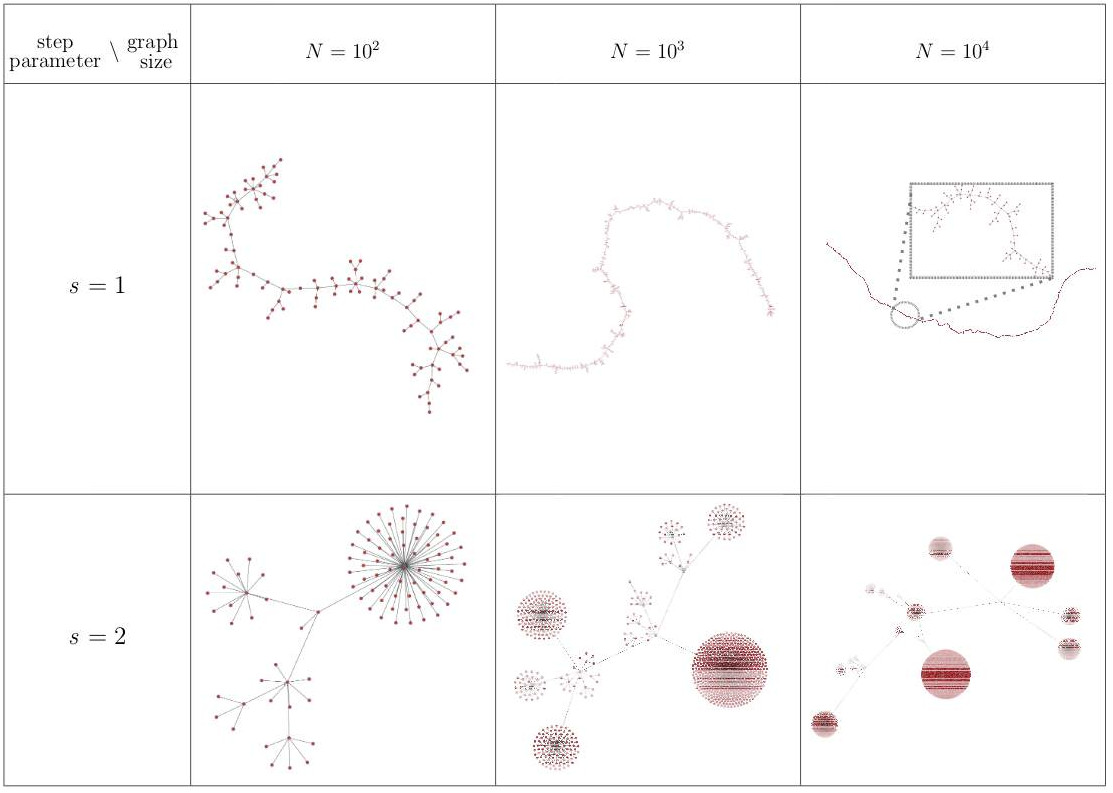
\includegraphics[width=.9\textwidth]{pictures/simulations.jpg}
   \caption{NRRW-prosessin realisaatioita tietokonesimulaatioissa. Kuva on kopioitu aiemmasta tutkimuksesta (Iacobelli et al.) [1]. \label{simulaatiot}}
\end{figure}

\subsection{Kaksi prosessia}

NRRW-prosessin ominaisuudet ovat seurausta satunnaiskulun ja sen kasvattaman satunnaisen verkon välisestä vuorovaikutuksesta. Malli on monimutkainen ja yksinkertaisuuden vuoksi on ensin syytä tarkastella satunnaisverkkoa ja satunnaiskulkua erillisinä prosesseina. Tämä mahdollistaa erillisiin malleihin liittyvän terminologian ja yksityiskohtien esittelyn ennen NRRW-prosessin kokonaisuuteen paneutumista.

\subsubsection{Satunnaisverkko}

Olkoon \( (\Grandom_{t}^{s})_{t \in \N_{0}} \) satunnaisverkko, johon lisätään uusi solmu \textit{s} aikayksikön välein. Jos verkon juurisolmussa esiintyvää silmukkaa ei huomioida, satunnaisprosessin tilajoukko on kaikkien suuntaamattomien, yhtenäisten ja syklittömien verkkojen eli puiden joukko.
\begin{definition}
   \label{definition:verkko}
Suuntaamaton verkko $ G $ on pari $ (V, E) $, missä joukko $ V $ on verkon solmujen joukko (\( v_{i} \in V \)) ja $ E $ on suuntaamattomien kaarien joukko. Kaarien joukon alkiot ovat muotoa \( \{ v_{i}, v_{j} \} \). Kaari \( \{ v_{i}, v_{j} \} \) yhdistää solmut \( v_{i} \) ja \( v_{j} \) toisiinsa. 
\end{definition}
Kasvavan verkon käsittelyn helpottamiseksi satunnaisverkon \( (\Grandom_{t}^{s})_{t \in \N_{0}} \) solmut indeksoidaan kokonaisluvuilla (\( 0, 1, 2, \ldots \)) lisäysjärjestyksen mukaan. Juurisolmu on siis \( v_{0} \) ja hetkellä \( t = sn \) (\( n \in \N_{0} \)) lisätään solmu \( v_{n} \). Jos satunnaisverkkoa \( (\Grandom_{t}^{s})_{t \in \N_{0}} \) tarkastellaan itsenäisenä prosessina, sen siirtymätodennäköisyydet pois nykytilasta ovat nollasta poikkeavia vain ajanhetkillä \( s\N_{0} = \left\{ sn \: : \: n \in \N_{0} \right\} \). Silloin ne määrää satunnaiskulun \( (\Wrandom_{t})_{t \in \N_{0}} \) siirtymämatodennäköisyydet:
\begin{equation}
   \setlength{\jot}{10pt}
   \begin{aligned}
   & \prob \left[ \Grandom_{t+s}^{s} = (V_{t} \cup \{ v_{j + 1} \}, E_{t} \cup \{ (v_{i}, v_{j + 1}) \}) \mid \Grandom_{t}^{s} = (V_{j}, E_{j}), \Wrandom_{t} = v_{j} \right] \\
   &= \prob \left[ \Wrandom_{t+s} = v_{i} \mid \Wrandom_{t} = v_{n}, G_{t} = (V_{t}, E_{t}) \right].
   \end{aligned}
\end{equation}

\subsubsection{Satunnaiskulku}

Vastaavasti satunnaiskulkuprosessin \( (\Wrandom_{t})_{t \in \N_{0}} \) tilajoukon ja siirtymätodennäköisyydet määrää sen kasvattama satunnaisverkko. Sekä tilajoukko että siirtymätodennäköisyydet muuttuvat aina, kun verkkoon lisätään uusi solmu. Lisäyshetkien välillä tilajoukko on kuitenkin vakio ja satunnaiskävelyprosessi voidaankin silloin nähdä tavallisena äärellisen tilajoukon Markov-ketjuna. Jos satunnaiskävely on solmussa \( v_{i} \) hetkellä \( t \), määräytyy seuraava tila satunnaisesti valitsemalla yksi solmusta \( v_{i} \) lähtevä kaari ja siirtymällä sen osoittamaan solmuun. Todennäköisyysmassa on tasajakautunut kaikkien solmun \( v_{i} \) kaarien kesken. 

Koska NRRW-prosessi rakentaa puita, ei verkossa ole muita syklejä kuin juuren kaari itseensä. Verkkoteoriassa kaaret solmusta itseensä lasketaan kahdesti, joten merkitään solmun \( v_{i} \) solmuun \( v_{j} \) yhdistävien kaarien määrää verkossa $ G_{i} $
\begin{equation}
   \psi_{G_{i}}(v_{i}, v_{j}) = 1 + \indicator \left\{ v_{i} = v_{0}, v_{j} = v_{0} \right\},
   \label{equation:psi}
\end{equation}
missä $ v_{0} $ on verkon $ G_{i} $ juurisolmu. Lauseke on perustuu siihen tosiasiaan, että NRRW-prosessi on juurisolmun silmukkaa lukuunottamatta sykliton. NRRW-prosessin kasvattama verkko on sellainen. Nyt todennäköisyys siirtyä solmusta \( v_{i} \) solmuun \( v_{j} \) verkossa $ G_{i} $ on yksinkertaisesti
\begin{equation}
   \prob \left[ \Wrandom_{t+1} = v_{j} \mid \Wrandom_{t} = v_{i}, \Grandom_{t}^{s} = G_{i} \right] = \frac{\psi_{G_{i}}(v_{i}, v_{j})}{d_{G_{i}}(v_{i})}.
   \label{equation:verkko-tn}
\end{equation}
Yllä \( d_{G_{i}}(v_{i}) \) merkitsee solmun \( v_{i} \) astelukua verkossa $ G_{i} $. Toisin sanoen
\begin{equation}
   d_{G_{i}}(v_{i}) = \sum_{w \in V_{i}} \psi_{G_{i}}(v_{i}, w)
   \label{equation:asteluku}
\end{equation}
on kaikkien solmuun \( v_{i} \) yhdistyvien kaarien lukumäärä.

\subsection{Kokonaisuus}

Satunnaisverkon ja satunnaiskulun erillinen tarkastelu paljastaa, että näistä jälkimmäinen on NRRW-prosessin todellinen satunnaisuuden lähde. Satunnaiskävely muuttaa liikkeillään sen omaa tilajoukkoa eli satunnaisverkkoa \( \Grandom_{t}^{s} \). Kun verkko muuttuu, myös satunnaiskävelyn siirtymätodennäköisyydet muuttuvat. Satunnaisverkko sen sijaan kasvaa satunnaiskävelyn realisaation ohjaamana. Kokonaisuutena NRRW-prosessi on siis ajassa epähomogeeninen äärettömän tilajoukon Markov-prosessi. Prosessin epähomogeenisuus juontaa siitä, että satunnaisverkko muuttuu vain $ s $:n ajanhetken välein.

\subsubsection{Tilajoukko}

Olkoon $ V = \left\{ v_{1}, v_{2}, \ldots \right\} $ kaikkien solmujen numeroituvasti ääretön joukko. Jos $ n $:n solmun joukkoa merkitään $ V_{n} = \{ v_{1}, v_{2}, \ldots , v_{n} \} \subset V $ niin $ n $:n solmun suuntaamattomien verkkojen joukko on
\[
   \mathbb{G}_{n} = \{ (V_{n}, E_{n}) \mid E_{n} \subset V_{n}^{2}  \},
\]
missä $ V_{n}^{2} = \left\{ e \subset V_{n} : |e| = 2 \right\} $ on solmujoukon $ V_{n} $ järjestämättömien parien joukko. NRRW-prosessiin kuuluu myös satunnaiskävely, jonka tilajoukko on $ n $:n solmun verkkoa kulkiessa verkon solmujen joukko $ V_{n} $. Selvästi $ n $:n solmun NRRW-prosessin tilajoukko on siis karteesinen tulo $ S_{n} = V_{n} \times \mathbb{G}_{n} $.

Merkitään kaikkien solmujen joukkoa numeroituvasti äärettömällä joukolla $ V $. Vastaavasti kaikkien verkkojen joukkoa voidaan merkitä äärettömällä unionilla
\begin{equation}
   \mathbb{G} = \bigcup_{n = 1}^{\infty} \mathbb{G}_{n}.
\end{equation}
Koska satunnaisverkko kasvaa NRRW-prosessin edetessä, täytyy sen tilajoukon sisältää kaikki eri solmulukumäärien mahdollistamat tilat. NRRW-prosessin tilajoukko onkin siis
\begin{equation}
   S = V \times \mathbb{G}.
   \label{equation:tilajoukko}
\end{equation}

\subsubsection{Siirtymätodennäköisyydet}

NRRW-prosessin siirtymätodennäköisyydet ovat ajassa epähomogeenisia, sillä satunnaiskävelyn realisaatio kasvattaa sen omaa tilajoukkoa, eli NRRW-prosessin verkkoa vain kun $ t \bmod s = 0 $. Siirtymätodennäköisyyksiä on siten syytä tarkastella kahdessa eri tapauksessa ajanhetken jaollisuuden mukaan. 

Olkoon $ (\Wrandom_{t}, \Grandom^{s}_{t}) $ NRRW-prosessi hetkellä $ t $ ja $ G = (V, E) \in \mathbb{G} $ sekä $ G' = (V', E') \in \mathbb{G} $ joitain NRRW-prosessin kasvattamia verkkoja. 
Jos $ v \in V $ ja $ v' \in V' $ ovat solmuja noissa verkoissa, niin NRRW-prosessin siirtymätodennäköisyydet saavat esityksen
\begin{equation}
   \setlength{\jot}{10pt}
   \begin{aligned}
      P\left( (v', G'), (v, G) \right) &= \prob \left[ (\Wrandom_{t+1}, \Grandom^{s}_{t+1}) = (v, G) \mid (\Wrandom_{t}, \Grandom^{s}_{t}) = (v', G') \right] \\
                                       &= \prob \left[ \Wrandom_{t+1} = v, \Grandom^{s}_{t+1} = G \mid \Wrandom_{t} = v', \Grandom^{s}_{t} = G' \right]
      \label{equation:siirtyma-tn}
   \end{aligned}
\end{equation}
{\parindent0pt
\textbf{Kun $ t + 1 \bmod s \neq 0, $} ei prosessin verkkoon lisätä uusia solmuja. Satunnaisverkko $ \Grandom^{s}_{t+1} $ on siis varmasti sama kuin sen edeltäjä $ \Grandom^{s}_{t} $. Siten
$ \prob \left[ \Grandom^{s}_{t+1} = G \mid \Grandom^{s}_{t} = G \right] = 1 $
riippumattomasti satunnaiskävelyn tilasta. Selvästi tapahtuman komplementti ($ \Grandom^{s}_{t+1} \neq G $) on mahdoton. Nyt yhtälön \ref{equation:siirtyma-tn} mukaisesti
\begin{equation*}
   \setlength{\jot}{10pt}
   \begin{aligned}
   P\left( (v', G'), (v, G) \right) &= \prob \left[ \Wrandom_{t+1} = v, \Grandom^{s}_{t+1} = G \mid \Wrandom_{t} = v', \Grandom^{s}_{t} = G' \right] \\
   &= \prob \left[ \Grandom^{s}_{t+1} = G \mid \Wrandom_{t} = v', \Grandom^{s}_{t} = G' \right] \\
   &\times \; \prob \left[ \Wrandom_{t+1} = v \mid \Wrandom_{t} = v', \Grandom^{s}_{t} = G', \Grandom^{s}_{t+1} = G \right] \\
   &= \prob \left[ \Grandom^{s}_{t+1} = G \mid \Grandom^{s}_{t} = G' \right] \prob \left[ \Wrandom_{t+1} = v \mid \Wrandom_{t} = v', \Grandom^{s}_{t} = G' \right] \\
   &= \indicator \left\{ G = G' \right\} \prob \left[ \Wrandom_{t+1} = v \mid \Wrandom_{t} = v', \Grandom^{s}_{t} = G' \right] \\
   &= \indicator \left\{ G_{i} = G_{j} \right\} \frac{\psi_{G_{i}}(v_{i}, v_{j})}{d_{G_{i}}(v_{i})}
   \end{aligned}
\end{equation*}
missä viimeinen yhtäsuuruus seuraa lausekkeesta \ref{equation:verkko-tn}.

\vspace{0.5cm}

\textbf{Kun $ t + 1 \bmod s = 0, $} satunnaisverkko $ \Grandom^{s}_{t+1} $ määräytyy satunnaiskävelyn $ \Wrandom_{t+1} $ realisaatiosta.
\begin{equation*}
   \setlength{\jot}{10pt}
   \begin{aligned}
   P\left( (v', G'), (v, G) \right) &= \prob \left[ \Wrandom_{t+1} = v, \Grandom^{s}_{t+1} = G \mid \Wrandom_{t} = v', \Grandom^{s}_{t} = G' \right] \\
   &= \prob \left[ \Wrandom_{t+1} = v \mid \Wrandom_{t} = v', \Grandom^{s}_{t} = G' \right] \\
   &\times \; \prob \left[ \Grandom^{s}_{t+1} = G \mid \Wrandom_{t+1} = v, \Wrandom_{t} = v', \Grandom^{s}_{t} = G' \right].
   \end{aligned}
\end{equation*}
Uusi solmu lisätään nyt siihen verkon $ G' $ solmuun, johon satunnaiskävely siirtyy ajanhetkellä $ t + 1 $. Selvästi mahdollisia satunnaisverkon $ \Grandom^{s}_{t+1} $ realisaatioita ovat vain sellaiset verkot, jotka on saatu liittämällä verkkoon $ G' $ yksi uusi solmu, $ v^{+} = v_{\lfloor \frac{t+1}{s} \rfloor} $. Kun verkkoja $ G $ ja $ G' $ merkitään verkon määritelmän (\ref{definition:verkko}) mukaisina solmujen ja kaarien pareina $ (V, E) $ ja $ (V', E') $,
\begin{equation*}
   \setlength{\jot}{10pt}
   \begin{aligned}
   P\left( (v', G'), (v, G) \right) &= \prob \left[ \Wrandom_{t+1} = v \mid \Wrandom_{t} = v', \Grandom^{s}_{t} = (V', E') \right] \\
           &\times \; \prob \left[ \Grandom^{s}_{t+1} = (V, E) \mid \Wrandom_{t+1} = v, \Wrandom_{t} = v', \Grandom^{s}_{t} = (V', E') \right] \\
           &= \indicator \left\{ (V, E) = (V' \cup \{ v^{+} \}, E' \cup \left\{ \left\{ v, v^{+} \right\} \right\}) \right\} \\
           &\times \; \prob \left[ \Wrandom_{t+1} = v' \mid \Wrandom_{t} = v', \Grandom^{s}_{t} = (V', E') \right] \\
           &= \indicator \left\{ G = (V' \cup \{ v^{+} \}, E' \cup \left\{ \left\{ v, v^{+} \right\} \right\}) \right\} \frac{\psi_{G'}(v, v')}{d_{G'}(v')},
   \end{aligned}
\end{equation*}
missä viimeinen yhtäsuuruus perustuu kaavaan \ref{equation:verkko-tn}.
}

\section{Stokastinen esitys}

NRRW-prosessin tarkastelu osoittaa, että kyseessä on monimutkainen ja epähomogeeninen äärettömän tilajoukon stokastinen prosessi. Sen käsittelyä voidaan kuitenkin helpottaa tukeutumalla
prosessin kanssa yhdenmukaiseen mutta yksinkertaisempaan malliin, NRRW-prosessin stokastiseen esitykseen.

\subsection{Yleistä teoriaa}

Olkoon \( (\omega_{t})_{t \geq 0} \) jono riippumattomia välin \( [0, 1] \) tasajakautuneita satunnaislukuja. Toisin sanoen \( \omega_{t} \sim \text{Tas}(0, 1) \). Tällaista satunnaislukujen sarjaa voidaan käyttää monimutkaisemman stokastisen prosessin algoritmiseen simulointiin. Simulointi rakennetaan etsimällä deterministinen funktio \( \phi : S \times [0, 1] \to S \), joka liittää stokastisen prosessin tilan ja välin \( [0, 1] \) reaaliluvun prosessin seuraavaan tilaan. Funktion \( \phi \) tulee toteuttaa $ \forall \; x, y \in S $ yhtälö
\begin{equation}
   \begin{aligned}
   \prob \left[ \phi(x, \omega_{t}) = y \right] &= \int\limits_0^1 \; \indicator \left\{ \phi(x, w) = y \right\} \mathrm{d}w \\
                                                &= \prob \left[ X_{t+1} = y \mid X_{t} = x \right] = P(x, y).
   \end{aligned}
   \label{equation:stokastinen-esitys}
\end{equation}
Yhtälön \ref{equation:stokastinen-esitys} toteuttavaa funktiota \( \phi \) ja satunnaislukujonoa \( (\omega_{t})_{t \geq 0} \) kutsutaan siirtymämatriisin P \textit{stokastiseksi esitykseksi}. Jos stokastisen prosessin alkutila on \( X_{0} = x_{0} \), sitä voidaan simuloida sen stokastisen esityksen avulla rekursiivisesti:
\[
   X_{t+1} = \phi(X_{t}, \omega_{t}).
\]
Mikäli stokastinen prosessi on epähomogeeninen ajassa, vaaditaan stokastiseen esitykseen jono deterministisiä funktioita \( (\phi^{(t)})_{t \geq 0} \), jotka ovat muotoa \( \phi^{(t)} : S \times [0, 1] \to S \). Funktioiden \( \phi^{(t)} \) tulee toteuttaa yhtälöä \ref{equation:stokastinen-esitys} vastaava ehto \( \forall \; t \geq 0 \; \text{ja} \; x, y \in S \):
\begin{equation}
   \prob \left[ \phi^{(t)}(x, \omega_{t}) = y \right] = \prob \left[ X_{t+1} = y \mid X_{t} = x \right] = P^{(t)}(x,y).
   \label{equation:epahom-stokastinen-esitys}
\end{equation}
Prosessin simulointi tehdään, kuten homogeenisessa tilanteessa, mutta rekursiofunktio valitaan funktiojonosta \( (\phi^{(t)})_{t \geq 0} \) järjestyksessä. \cite{Haggstrom}

\subsection{Prosessin esitys}

Edellä havaittiin, että NRRW-prosessi on epähomogeeninen ajassa. Sen stokastinen esitys on siis muotoa \( (\phi_{t}, \omega_{t})_{t \geq 0} \), missä funktiot \( \phi_{t} \) toteuttavat ehdon \ref{equation:epahom-stokastinen-esitys}. Muodostetaan sopiva jono deterministisiä funktioita NRRW-prosessille. Prosessin tilat ovat muotoa \( (v, G) \), missä \( G = (V, E) \) on verkko ja \( v \in V \) on verkon G solmu. Jakamalla rekursiofunktiot satunnaiskävely- ja satunnaisverkko-osiin saadaan niille korkeatasoinen muoto
\begin{equation}
   \phi^{(t)} \left( (v, G), w \right) = \left( \lambda\left( (v, G), w \right), \mu^{(t)} \left( \lambda\left( (v, G), w \right), G \right) \right),
   \label{equation:esitys-1}
\end{equation}
missä \( \lambda \) on satunnaiskulun \( (\Wrandom_{t})_{t \geq 0} \) stokastisen esityksen rekursiofunktio parametriksi annetussa verkossa G, ja \( \mu \) päivittää verkkoa G satunnaiskulun realisaation mukaisesti. Satunnaiskulun rekursiofunktio
\begin{equation}
   \lambda \left( (v_{i}, G), w \right) = 
   \begin{cases}
      v_{1} & w \in [0, \rho(G)_{i,1}) \\
      v_{2} & w \in [\rho(G)_{i,1}, \rho(G)_{i,1} + \rho(G)_{i,2}) \\
            & \quad \vdots \\
      v_{\mid V \mid} & w \in [\rho(G)_{i,\mid V \mid - 1}, \rho(G)_{i,\mid V \mid - 1} + \rho(G)_{i,\mid V \mid}) 
   \end{cases},
   \label{equation:esitys-kulku}
\end{equation}
missä \( \rho \) on funktio verkosta sen siirtymämatriisiin (\ref{equation:esitys-siirt}) ja $ |V| $ on verkon $ G $ solmujen lukumäärä. Hyödyntäen kaavan \ref{equation:psi} esitystä solmuja yhdistävien kaarien määrälle saadaan kuvaukselle \( \rho \) alkioittainen määritelmä
\begin{equation}
   \rho(G)_{i,j} = \frac{\psi_{G}(v_{i}, v_{j})}{d_{G}(v_{i})} = \frac{1 + \indicator \left\{ v_{i} = v_{0}, v_{j} = v_{0} \right\}}{d_{G}(v_{i})},
   \label{equation:esitys-siirt}
\end{equation}
joka vastaa aiemmin laskettuja satunnaiskulun $ (\Wrandom_{t})_{t \in \N_{0}} $ siirtymätodennäköisyyksiä (kaava \ref{equation:verkko-tn}). Lopuksi stokastisen esityksen verkkoa päivittävä funktio
\begin{equation}
   \mu^{(t)} \left( v, (V, E) \right) =
   \begin{cases}
      \left( V \cup \{v_{t/s}\}, E \cup \left\{ \{ v, v_{t/s} \} \right\} \right) & \text{kun } t \bmod s = 0 \\
      \left( V, E \right) & \text{muulloin}
   \end{cases}.
   \label{equation:esitys-4}
\end{equation}
Funktio lisää solmuun \( v \) uuden solmun \( v_{t/s} \) aina, kun aika, $ t $, on jaollinen askelparametrillä s. Muulloin verkkoa ei muuteta.

\begin{theorem}
Olkoon $ (\omega_{t})_{t \geq 0} $ jono riippumattomia välin $ [0, 1] $ tasajakautuneita satunnaislukuja. Kaavojen \ref{equation:esitys-1}-\ref{equation:esitys-4} määrittelemä jono deterministisiä funktioita $ (\phi^{t})_{t \geq 0} $ muodostaa yhdessä satunnaislukujonon $ (\omega_{t})_{t \geq 0} $ kanssa NRRW-prosessin stokastisen esityksen.
\label{theorem:my-theorem}
\end{theorem}
\begin{proof}
NRRW-prosessin siirtymätodennäköisyydet on laskettu kappaleessa 2.3.1. Prosessin käyttäytyminen ajanhetkellä $ t $ riippuu siitä, onko $ t $ jaollinen askelparametrilla $ s $. Osoitetaan stokastisen esitykseen yhdenmukaisuus NRRW-prosessin kanssa molemmissa tapauksissa. Olkoon $ X_{t} = (\Wrandom_{t}, \Grandom^{s}_{t}) $ NRRW-prosessin tila hetkellä $ t $. 

On näytettävä kaavan \ref{equation:epahom-stokastinen-esitys} mukaisesti, että
\[
   \prob \left[ \phi^{(t)}(x, \omega_{t}) = y \right] = \prob \left[ X_{t+1} = y \mid X_{t} = x \right] 
\]
kaikilla $ x, y \in S $ ja $ t \in \N_{0} $, missä $ S $ on kaavan \ref{equation:tilajoukko} määrittelemä NRRW-prosessin tilajoukko. Sijoittamalla aiemmin määritelty stokastinen esitys yhtälön vasempaan puoleen saadaan
\begin{align*}
   \prob \left[ \phi^{(t)}(x, \omega_{t}) = y \right] &= \int\limits_0^1 \; \indicator \left\{ \phi^{(t)}(x, w) = y \right\} \mathrm{d}w \\
                                                &= \int\limits_0^1 \; \indicator \left\{ \left( \lambda\left( (v_{x}, G_{x}), w \right), \mu^{(t)} \left( \lambda\left( (v_{x}, G_{x}), w \right), G_{x} \right) \right) = (v_{y}, G_{y}) \right\} \mathrm{d}w \\
                                                &= \int\limits_0^1 \; \indicator \left\{ \lambda\left( (v_{x}, G_{x}), w \right) = v_{y} \right\} \indicator \left\{ \mu^{(t)} \left( \lambda\left( (v_{x}, G_{x}), w \right), G_{x} \right) = G_{y} \right\} \mathrm{d}w
\end{align*}

\paragraph{Kun $ t + 1 \bmod s \neq 0 $},
\begin{align*}
   \prob \left[ \phi^{(t)}(x, \omega_{t}) = y \right] &= \int\limits_0^1 \; \indicator \left\{ \lambda\left( (v_{x}, G_{x}), w \right) = v_{y} \right\} \indicator \left\{ \mu^{(t)} \left( \lambda\left( (v_{x}, G_{x}), w \right), G_{x} \right) = G_{y} \right\} \mathrm{d}w \\
                                                &= \indicator \left\{ G_{x} = G_{y} \right\} \int\limits_0^1 \; \indicator \left\{ \lambda\left( (v_{x}, G_{x}), w \right) = v_{y} \right\} \mathrm{d}w \\
                                                &= \indicator \left\{ G_{x} = G_{y} \right\} \rho(G_{x})_{x,y} = \indicator \left\{ G_{x} = G_{y} \right\} \frac{\psi_{G_{x}}(v_{x}, v_{y})}{d_{G_{x}}(v_{x})} \\
                                                &= \prob \left[ X_{t+1} = y \mid X_{t} = x \right].
\end{align*}

\paragraph{Kun $ t + 1 \bmod s = 0 $},

\begin{align*}
   \prob \left[ \phi^{(t)}(x, \omega_{t}) = y \right] &= \int\limits_0^1 \; \indicator \left\{ \lambda\left( (v_{x}, G_{x}), w \right) = v_{y} \right\} \indicator \left\{ \mu^{(t)} \left( \lambda\left( (v_{x}, G_{x}), w \right), G_{x} \right) = G_{y} \right\} \mathrm{d}w \\
                                                &= \indicator \left\{ G_{y} = (V_{x} \cup \{ v_{y} \}, E_{x} \cup \left\{ \{ v_{x}, v_{y} \} \right\}) \right\} \int\limits_0^1 \; \indicator \left\{ \lambda\left( (v_{x}, G_{x}), w \right) = v_{y} \right\}  \mathrm{d}w \\
                                                &= \indicator \left\{ G_{y} = (V_{x} \cup \{ v_{y} \}, E_{x} \cup \left\{ \{ v_{x}, v_{y} \} \right\}) \right\} \rho(G_{x})_{x,y} \\
                                                &= \indicator \left\{ G_{y} = (V_{x} \cup \{ v_{y} \}, E_{x} \cup \left\{ \{ v_{x}, v_{y} \} \right\}) \right\} \frac{\psi^{(t)}(v_{i}, v_{j})}{d_{t}(v_{i})} \\
                                                &= \prob \left[ X_{t+1} = y \mid X_{t} = x \right].
\end{align*}
Selvästi kaikilla $ t \in \N_{0} $ pätee, että $ \prob \left[ \phi^{(t)}(x, \omega_{t}) = y \right] = \prob \left[ X_{t+1} = y \mid X_{t} = x \right] $. Siten rakentamani stokastinen esitys on ekvivalentti NRRW-prosessin kanssa.

\end{proof}

\section{Parillinen prosessi}

\begin{figure}[htb]
\centering
\includegraphics[width=.8\textwidth]{pictures/simulation_4_50000.png}
   \caption{Tietokonesimuloitu NRRW-prosessi parillisella askelparametrilla $ s = 4 $. \label{figure:oma_simulaatio}}
\end{figure}

NRRW-prosessin käyttäytymiseen vaikuttaa voimakkaasti askelparametrin $ s $ parillisuus. Parillisen parametrin prosessissa satunnaiskävely $ (\Wrandom_{t})_{t \in \N_{0}} $ on palautuva, eli se vierailee kaikissa sen tilajoukon solmuissa äärettömän monta kertaa lähes varmasti. Sen sijaan ainakin askelparametrin $ s = 1 $ satunnaiskulku on väistyvä. Askelparametrin parillisuus vaikuttaa yhtä radikaalisti satunnaisverkkojen ominaisuuksiin. Parillisen askelparametrin satunnaisverkon $ (\Grandom^{s}_{t})_{t \in \N_{0}} $ sisäsolmujen astelukujen jakauma on potenssilain alhaalta rajoittama, kun taas askelparametrin $ s = 1 $ solmujen astelukujen jakauma on geometrisen jakauman ylhäältä rajoittama.

Erityisesti vain parillisen askelparametrin NRRW-prosessissa kaksi peräkkäistä uutta solmua voidaan lisätä samaan verkon solmuun. Parittoman askelparametrin prosessissa tämä ei ole mahdollista muualla kuin puun juuressa, sillä satunnaiskulku siirtyy $ s $:ssä askeleessa puun parittomalta tasolta parilliselle ja toisinpäin. Merkitään satunnaiskulun tasoa ajanhetkellä $ t $ funktiolla $ d(\Wrandom_{t}, v_{0}) $, missä $ v_{0} $ on juurisolmu.
\begin{definition}
NRRW-prosessi ja sen satunnaiskulku $ \Wrandom_{t} $ ovat parillisia ajanhetkellä $ t $ $ \Leftrightarrow $ $ d(\Wrandom_{t}, r) + t $ on parillinen. Jos prosessi ei ole parillinen, se on pariton.
\label{definition:parity}
\end{definition}
Selvästi parillisen askelparametrin prosessin pariteetti muuttuu vain, kun satunnaiskulku kulkee puun juuren silmukan läpi.

Uuden, peräkkäisen solmun lisääminen samaan solmuun parillisessa NRRW-verkossa on paitsi mahdollista niin myös sitä todennäköisempää mitä suurempi kyseisen solmun asteluku on. Koska uusia solmuja lisätään erityisesti saman pariteetin tasoille puussa, jäävät uudet solmut lehdiksi (eng. leaf), kunnes prosessin pariteetti vaihtuu. Lehtisolmuista voi siirtyä vain takaisin lähtöpisteeseen, joten todennäköisyys palata johonkin satunnaisverkon solmuun suurenee, kun solmussa vieraillaan ja sen asteluku kasvaa. Kuva \ref{figure:oma_simulaatio} havainnollistaa, kuinka lehtisolmuja kasaantuu tähtimaiseen muodostelmaan joidenkin solmujen ympärille.

Tämä parillisen prosessin ominaisuus liittyy vahvasti suosivaan kiinnittymiseen, sillä uusia solmuja kertyy erityisen todennäköisesti sellaisille verkon solmuille, joilla on jo ennestään paljon naapureita. Kuten aiemmin on todettu, suosiva kiinnittyminen on tosielämän verkkorakenteiden kannalta kiinnostava ominaisuus. Käsite on yhteydessä sosiologiseen Matteus-efektiin, joka tarkoittaa etujen kasaantumista niille, joilla niitä on jo ennestään. Efektin ydinajatus tiivistetään usein lausahdukseen: "Rikkaat rikastuu ja köyhät köyhtyy". Keskitynkin tässä kandidaatintyössä parillisen NRRW-prosessin ominaisuuksia käsittelemiseen.

\subsection{Astelukujen jakauma}

\begin{figure}[htb]
\centering
   \begin{subfigure}[b]{0.47\textwidth}
      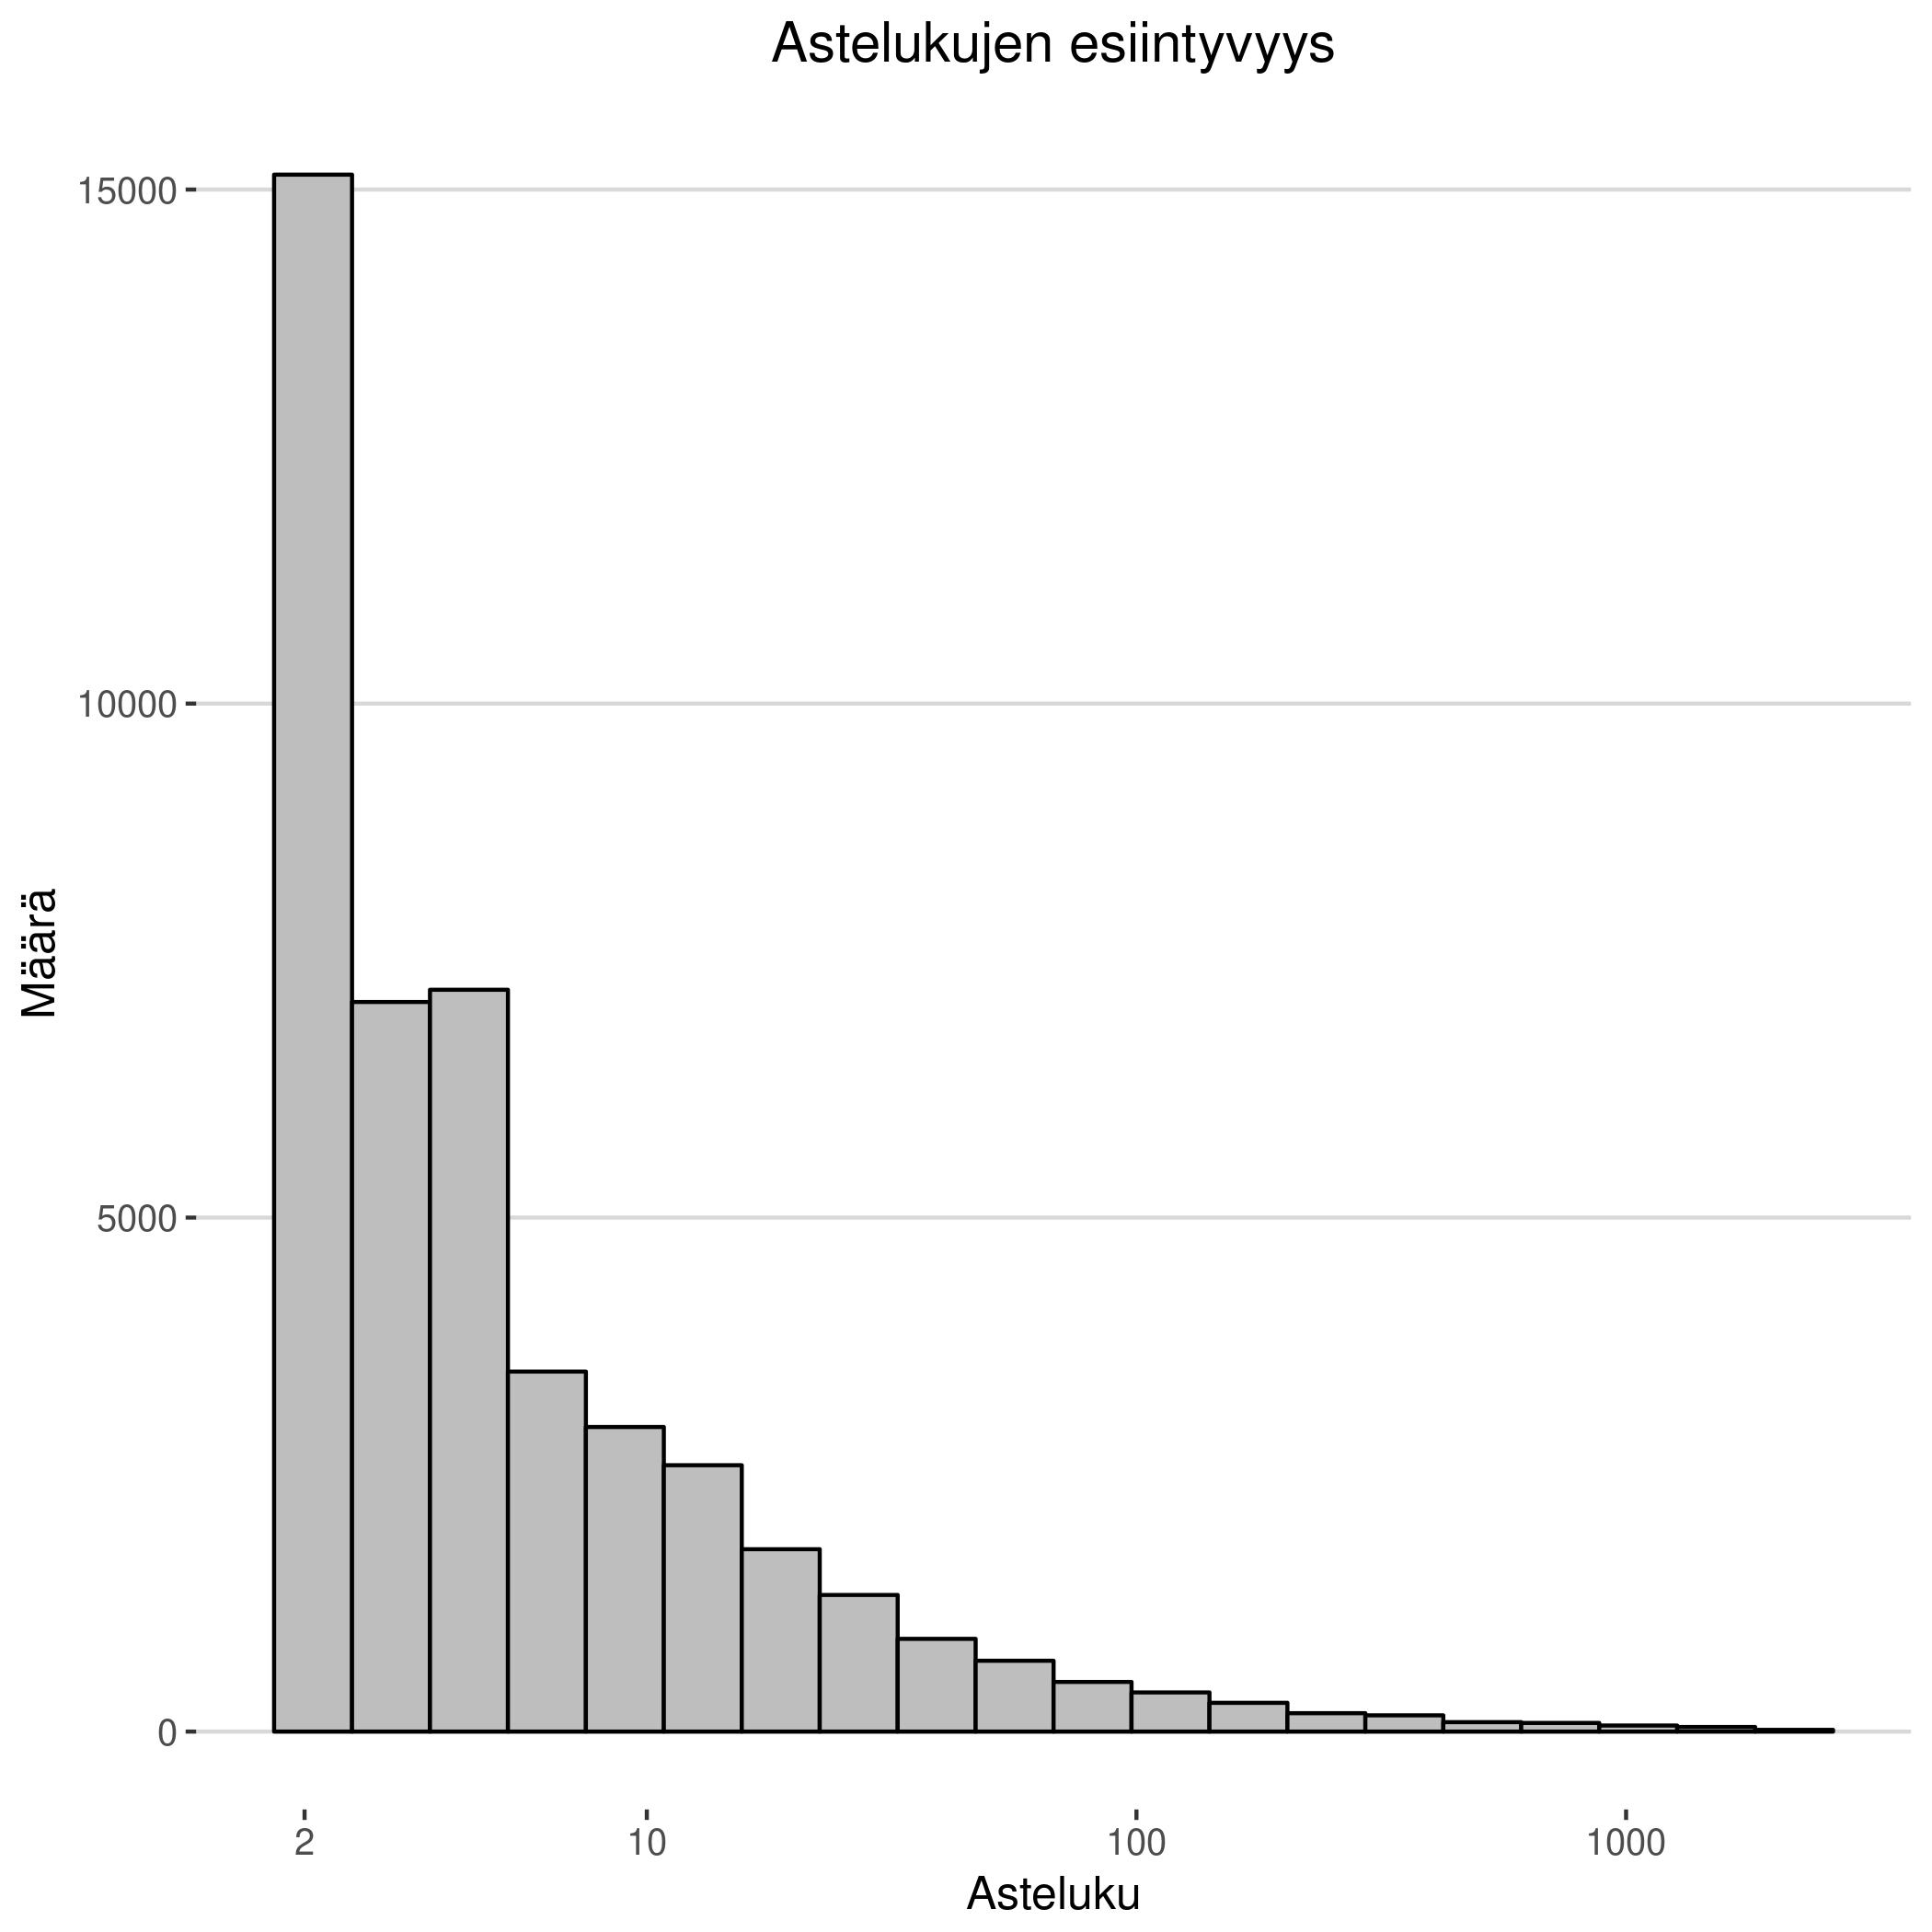
\includegraphics[width=\textwidth]{pictures/approx_hist.jpg}
      \caption{Sisäsolmujen astelukujen jakaumalla on raskaan näköinen häntä (eng. heavy tail). Histogrammin luokitus ei ole tasavälinen ja astelukuakseli on logaritminen. \label{figure:approx_hist}}
   \end{subfigure}
   \quad
   \begin{subfigure}[b]{0.47\textwidth}
      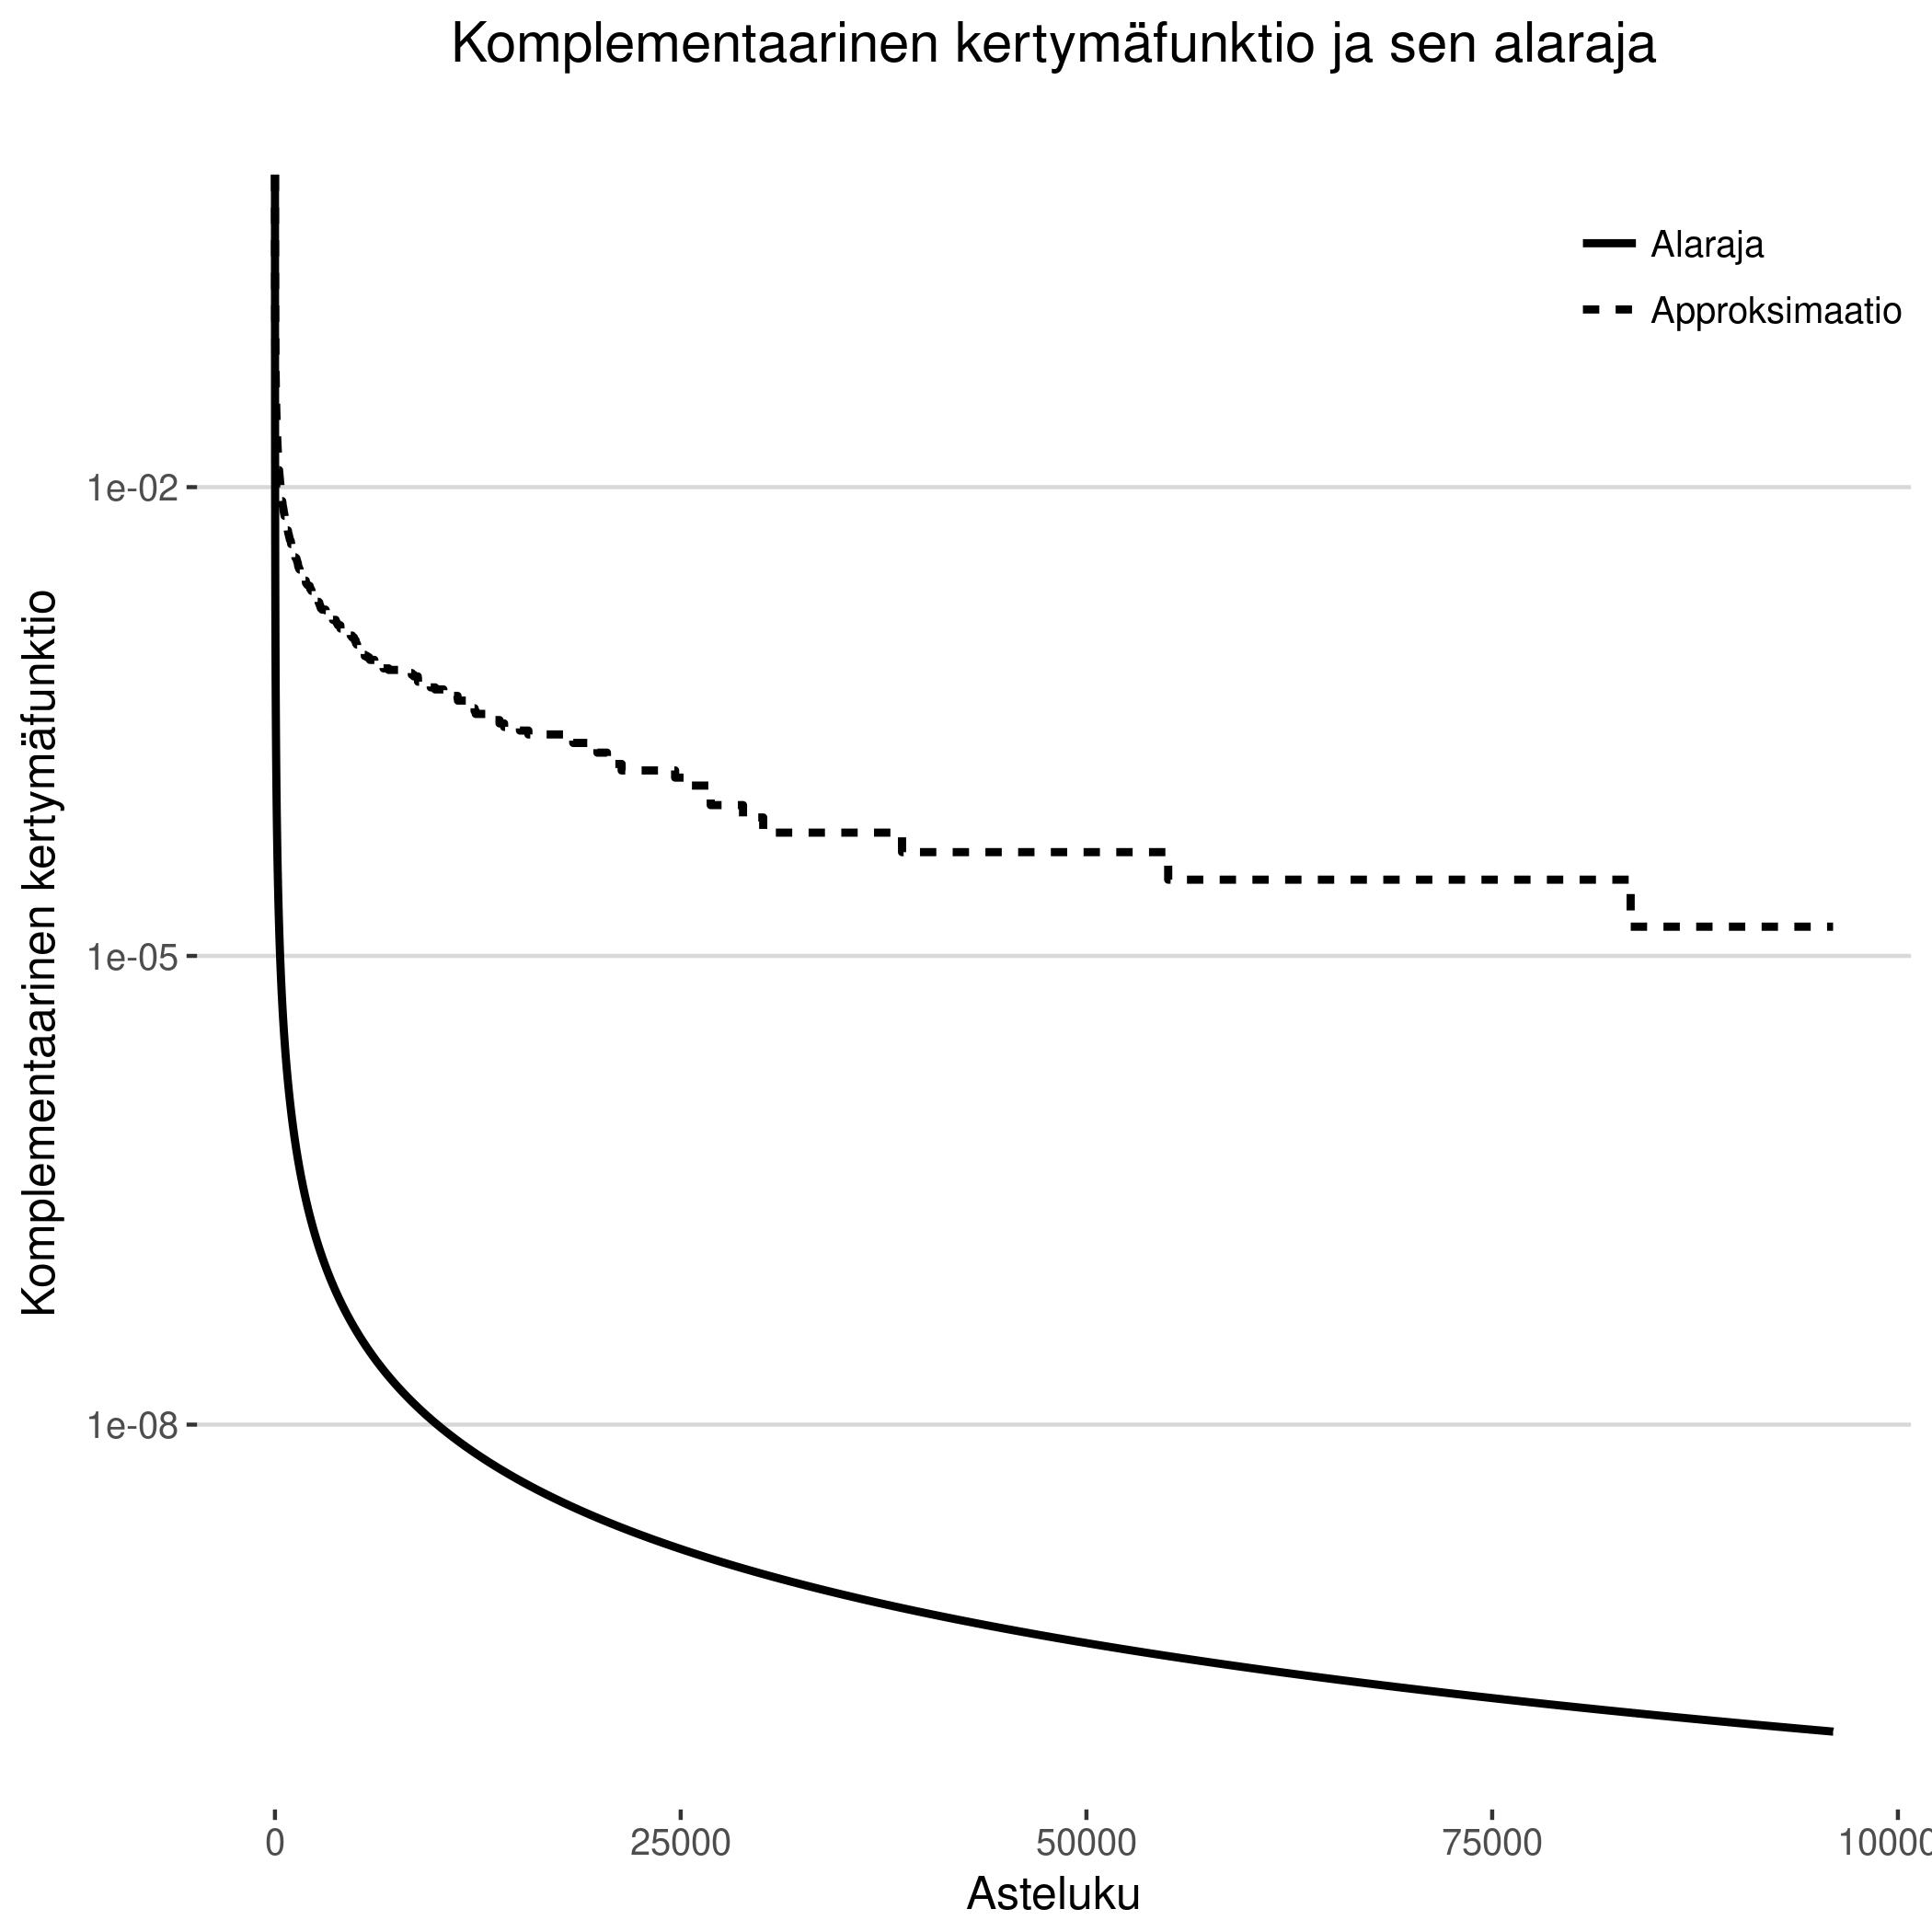
\includegraphics[width=\textwidth]{pictures/approx_cdf.jpg}
      \caption{Lauseen \ref{theorem:asteluku} mukainen alaraja vaikuttaa simulaatioiden perusteella uskottavalta. Empiirisen kertymäfunktion lisäksi kuvaajaan on piirretty kertymäfunktion estimaatti. Akselit ovat logaritmisia. \label{figure:approx_cdf}}
   \end{subfigure}
   \caption{Kuusitoista simuloitua NRRW-prosessia ($ s = 4 $) tuotti yhteensä 2400000 solmun otoksen. Solmuista 45077 oli sisäsolmuja.}
   \label{figure:asteluku-sim}
\end{figure}

Parillisen askelparametrin ja askelparametrin $ s = 1 $ NRRW-prosessit generoivat hyvin erilaisia verkkoja. Ehkä tärkein ero prosessien rakentamien verkkojen välillä liittyy sisäsolmujen
astelukujen jakaumiin. Parillinen prosessi nimittäin rakentaa verkkoja, joissa sisäsolmujen astelukujen jakauma on potenssilain alhaalta rajoittama (eng. heavy tail), kun taas parametrin $ s = 1 $ vastaava jakauma on geometrisen jakauman ylhäältä rajoittama (eng. exponential tail). Parillisen prosessin jakauma mukailee erityisesti lauseen \ref{theorem:asteluku} alarajaa \cite{Iacobelli}.

\begin{theorem}
   Olkoon NRRW-prosessin askelparametri $ s $ parillinen. Oletetaan, että $ T_{j} $ on se ajanhetki, jolloin solmuun $ j $ lisätään sen ensimmäinen naapuri. Tällöin kaikilla $ t \geq T_{j} $ ja $ k \in \{1,\ldots,\lfloor \frac{t-T_{j}}{s} \rfloor + 1\} $ pätee, että
   \[
      \renewcommand{\arraystretch}{2.0}
      \begin{array}{lr}
         \prob \left[ d_{t}(j) \geq k + 1 \mid T_{j} < \infty \right] \geq k^{-\frac{s}{2}},             & \text{jos} \; j \neq \text{juuri} \\
         \prob \left[ d_{t}(j) \geq k + 2 \right] \geq \left( \frac{k(k+1)}{2} \right)^{-\frac{s}{2}},   & \text{jos} \; j = \text{juuri}
      \end{array}
   \]
   \label{theorem:asteluku}
\end{theorem}
Arvioidakseni lauseen \ref{theorem:asteluku} uskottavuutta simuloin rinnakkain kuudentoista askelparametrin $ s = 4 $ NRRW-prosessin kehitystä 600000 askeleen päähän alkutilasta. 
Simulaatio-ohjelman lähdekoodi löytyy liitteestä A. Kuvaaja \ref{figure:asteluku-sim} esittää simuloidun otoksen sisäsolmujen astelukujen jakaumaa (\ref{figure:approx_hist}) ja 
vertaa sisäsolmujen empiiristä kertymäfunktiota $ \bar{F}_{n} $ lauseen \ref{theorem:asteluku} mukaiseen alarajaan (\ref{figure:approx_cdf}). Huomaa, että kuvaajan \ref{figure:approx_cdf}
funktiot ovat komplementaarisia kertymäfunktioita ($ \bar{F}(k) = 1 - F(k) $) perinteisen kertymäfunktion $ F $ sijaan. 

Koska kuvaajan \ref{figure:approx_cdf} käyrät näyttävät potenssilain mukaisilta, sovitin empiiriseen kertymäfunktioon $ \bar{F}_{n} $ mallin $ \hat{\bar{F}}(k) = k^{-b} $. Epälineaarinen
regressio estimoi parametrille $ b $ arvon $ \hat{b} \approx \frac{3}{4} $. Selvästikään lauseen \ref{theorem:asteluku} alaraja ei ole kovin hyvä ainakaan NRRW-prosessin askelparametrilla 
$ s = 4 $. Yhden askelparametrin simulaatiotuloksista ei kuitenkaan voi tehdä sellaista johtopäätöstä, että alaraja olisi heikko kaikilla parillisen askelparametrin prosesseilla.

\begin{table}[htb]
   \begin{center}
   \renewcommand{\arraystretch}{1.2}
   \begin{tabular}{|c|c|c|c|c|c|}
   \hline
   $ s           $ & 2     & 4     & 6     & 8     & 10 \\ \hline
   $ s / 2       $ & 1     & 2     & 3     & 4     & 5 \\ \hline
   $ \hat{b}     $ & 0.645 & 0.752 & 0.910 & 0.814 & 0.870 \\ \hline
   \end{tabular}
   \end{center}
   \caption{Sisäsolmujen astelukujen jakauman alaraja näyttää heikkenevän askelparametrin kasvaessa.}
   \label{table:bound-test}
\end{table}
Hahmottaakseni alarajan vahvuutta tarkemmin ajoin lyhyet simulaatiot viidellä eri parillisella askelparametrilla (2, 4, 6, 8 ja 10) ja vertasin lauseen \ref{theorem:asteluku} 
alarajaa estimoituihin, komplementaarisiin kertymäfunktioihin, $\hat{\bar{F}}$. Taulukko \ref{table:bound-test} esittää, miten estimoitu potenssi, $ \hat{b} $, kehittyy alarajan 
potenssin, $ \frac{s}{2} $, funktiona. Alaraja näyttää heikkenevän askelparametrin kasvaessa. Kaiken kaikkiaan vaikuttaakin siltä, että lauseen \ref{theorem:asteluku} alaraja 
on melko heikko. Vahvemman alarajan löytäminen ja sen oikeaksi osoittaminen on mahdollinen jatkotutkimuksen aihe.

\subsection{Palautuvuus}

Parillisessa NRRW-prosessissa pariteetin (määritelmä \ref{definition:parity}) vaihtumisella on tärkeä rooli prosessin rakentaman verkon kasvussa. Koska uusia solmuja lisätään
vain parillisille (tai parittomille) tasoille, kunnes prosessin pariteetti vaihtuu, näihin vasta lisättyihin solmuihin, jotka kuuluvat parittomalle (tai parilliselle) tasolle,
ei voida liittää uusia naapureita ennen kuin prosessin pariteetti vaihtuu. Tämä tarkoittaa sitä, että satunnaiskulun pariteetin on vaihduttava, jotta sen rakentaman puun korkeus kasvaisi. 

Selvästi satunnaisverkon korkeus jää äärelliseksi, mikäli satunnaiskulun pariteetti vaihtuu vain äärellisen monta kertaa. Jotta satunnaiskulun pariteetti vaihtuisi äärettömän monta kertaa
ja sen kasvattaman verkon korkeus olisi rajoittamaton, on satunnaiskulun vierailtava juurisolmussa äärettömän monta kertaa. Ainakin juurisolmun on siis oltava palautuva tila. Myöhemmin
näemme, että peräti kaikki NRRW-verkon solmut ovat palautuvia. Ennen sitä osoitan kuitenkin lemman \ref{lemma:recurrence}, joka liittää satunnaiskulun vierailut johonkin solmuun 
satunnaiskulun vierailuihin sen naapureissa. Hyödynnän todistuksessa toista Borelin-Cantellin lemmaa, joka on yksi todennäköisyysteorian keskeisimpiä lauseita.
\begin{lemma}[Toinen Borelin-Cantellin lemma]
   Olkoon $ E_{1}, E_{2}, \ldots $ jono riippumattomia tapahtumia jossain todennäköisyysavaruudessa. Jos jonon tapahtumien todennäköisyyksien summa on ääretön, eli
   \[
      \sum_{n = 1}^{\infty} \prob \left[ E_{n} \right] = \infty,
   \]
   niin todennäköisyys, että tapahtumia sattuu äärettömän monta on yksi:
   \[
      \prob \left[ \limsup \limits_{n \rightarrow \infty} E_{n} \right] = 1,
   \]
   missä $ \limsup \limits_{n \rightarrow \infty} E_{n} = \bigcap_{n = 1}^{\infty} \bigcup_{k \geq n}^{\infty} E_{k} $ on tapahtumajonon $ \{ E_{n} \}_{n=1}^{\infty} $ limit supremum. \text{\cite{Borel-Cantelli}}
\label{lemma:borel-cantelli}
\end{lemma}

Lemman \ref{lemma:recurrence} todistus mukailee aiemmassa tutkimuksessa (Iacobelli et al. \cite{Iacobelli}) rakennettua todistusta, mutta hyödynnän siinä itse rakentamaani NRRW-prosessin 
stokastista esitystä ja paikkaan aiemman todistuksen puutteita.
\begin{lemma}
Olkoon $ v_{i} $ solmu ja $ \{v_{i}, v_{j}\} $ kaari NRRW-prosessin verkossa. Jos $ v_{i} $ on palautuva, niin satunnaiskävely $ (\Wrandom_{t})_{t \in \N_{0}} $ kulkee kaaren $ \{v_{i}, v_{j}\} $ läpi äärettömän monta kertaa lähes varmasti.
\label{lemma:recurrence}
\end{lemma}

\begin{proof}
   Määritellään aluksi apufunktiot
   \begin{align*}
      J_{t_{1}}^{t_{2}}(v_{i})         &= \sum_{k = t_{1}}^{t_{2}} \indicator \left\{ \Wrandom_{k} = v_{i} \right\} \\
      J_{t_{1}}^{t_{2}}(v_{i}, v_{j})  &= \sum_{k = t_{1}}^{t_{2}} \indicator \left\{ \Wrandom_{k} = v_{i} \right\} \indicator \left\{ \Wrandom_{k+1} = v_{j} \right\}.
   \end{align*}
   Funktion $ J_{t_{1}}^{t_{2}}(v_{i}) $ arvo kertoo, kuinka usein satunnaiskulku $ (\Wrandom_{t})_{t \in \N_{0}} $ vierailee solmussa $ v_{i} $ ajanhetkien $ t_{1} $ ja $ t_{2} $ välillä.
   Vastaavasti $ J_{t_{1}}^{t_{2}}(v_{i}, v_{j}) $ ilmaisee, montako kertaa satunnaiskulku siirtyy solmusta $ v_{i} $ solmuun $ v_{j} $ kaaren $ \{ v_{i}, v_{j} \} $ läpi.
   Oletuksen mukaan solmu $ v_{i} $ on palautuva. Tämä tarkoittaa sitä, että NRRW-prosessin satunnaiskulku palaa äärellisessä ajassa takaisin solmuun $ v_{i} $ riippumatta satunnaisverkon
   $ \Grandom_{t}^{s} $ tilasta. Jos ensimmäinen siirtymähetki solmuun $ v_{i} $ määritellään
   \[
      T_{v_{i}}^{+} = \min \left\{ t \geq 1 : \Wrandom_{t} = v_{i} \right\}
   \]
   niin solmulle $ v_{i} $ pätee kaikilla oletuksen mukaisilla verkoilla $ G $, että
   \[
      \prob \left[ T_{v_{i}}^{+} < \infty \mid (\Wrandom_{t}, \Grandom_{t}^{s}) = (v_{i}, G) \right] = 1.
   \]
   Jos paluuaika solmuun $ v_{i} $ on äärellinen lähes varmasti, niin on selvää, että solmusta $ v_{i} $ käynnistyvä satunnaiskulku $ (\Wrandom_{t})_{t \in \N_{0}} $ myös vierailee
   rajoittamattoman ajanjakson aikana äärettömän monta kertaa solmussa $ v_{i} $:
   \begin{equation}
      \prob \left[ J_{0}^{\infty} = \infty \mid (\Wrandom_{t}, \Grandom_{t}^{s} = (v_{i}, G) \right] = 1.
      \label{equation:oletus}
   \end{equation}
   Olkoon $ (v', G') $ nyt mikä tahansa NRRW-prosessin tila, joka on saavutettavissa ajanhetkellä $ t $ ($ \prob \left[ (\Wrandom_{t}, \Grandom_{t}^{s}) = (w, G) \right] > 0 $).
   Koska NRRW-prosessin satunnaiskävely on yhtenäinen, satunnaiskulku $ (\Wrandom_{t})_{t \in \N_{0}} $ vierailee solmussa $ v_{i} $ äärettömän monta kertaa lähes varmasti riippumatta 
   siitä, mistä ajanhetkellä $ t $ saavutettavasta tilasta se käynnistyy. Toisin sanoen $ \prob \left[ J_{t}^{\infty}(v_{i}) = \infty \mid (\Wrandom_{t}, \Grandom_{t}) = (v', G') \right] = 1 $.
   Jos näin ei olisi, niin
   \[
      \begin{split}
      & \prob \left[ J_{0}^{\infty} < \infty \mid (\Wrandom_{t}, \Grandom_{t}^{s}) = (v_{i}, G) \right] \\
      & \quad > \prob \left[ J_{t}^{\infty}(v_{i}) < \infty \mid (\Wrandom_{t}, \Grandom_{t}^{s}) = (v', G') \right] \\
      & \quad \times \prob \left[ (\Wrandom_{t}, \Grandom_{t}^{s}) = (v', G') \mid (\Wrandom_{t}, \Grandom_{t}^{s}) = (v_{i}, G) \right] > 0,
      \end{split}
   \]
   mikä on ristiriita sen oletuksen kanssa, että $ v_{i} $ on palautuva.

   Olkoon $ t_{0} $ nyt sellainen ajanhetki, jolloin solmut $ v_{i} $ ja $ v_{j} $ sekä niitä yhdistävä kaari $ \{ v_{i}, v_{j} \} $ kuuluvat verkkoon $ \Grandom_{t_{0}}^{s} = G_{0} $.
   Lemman väite on nyt tosi, jos $ \prob \left[ J_{t_{0}}^{\infty}(v_{i}, v_{j}) = \infty \right] = 1. $ Todistetaan tämä hyödyntäen NRRW-prosessin stokastista esitystä.

   Olkoon $ (\omega_{t})_{t \geq t_{0}} $ jono riippumattomia välin $ [0, 1] $ tasajakutuneita satunnaislukuja. Kuten lause \ref{theorem:my-theorem} osoittaa, tällaista satunnaislukujen
   jonoa voidaan käyttää koko NRRW-prosessin $ (\Wrandom_{t}, \Grandom_{t}^{s}) $ simulointiin kaikilla $ t \geq t_{0} $. Erityisesti sen avulla voidaan määrittää, siirtyykö satunnaiskulku
   solmusta $ v_{i} $ solmuun $ v_{j} $ ajanhetkellä $ t $. Määritellään tätä varten uusi jono satunnaislukuja:
   \begin{equation*}
      \setlength{\jot}{10pt}
      \begin{aligned}
      \xi_{t} &= \indicator \left\{ \lambda((v_{i}, G_{t}), \omega_{t}) = v_{j} \right\} \\
              &= \indicator \left\{ \omega_{t} \in \left[ \rho(G_{t})_{i,j-1}, \rho(G_{t})_{i,j-1} + \rho(G_{t})_{i,j} \right] \right\} \\
              &= \indicator \left\{ \omega_{t} \in \left[ 0, \frac{\psi_{G_{t}}(v_{i}, v_{j})}{d_{G_{t}}(v_{i})} \right] \right\} 
              = \indicator \left\{ \omega_{t} \in \left[ 0, \frac{1 + \indicator \{ v_{i} = v_{0}, v_{j} = v_{0} \}}{d_{G_{t}}(v_{i})} \right] \right\},
      \end{aligned}
   \end{equation*}
   missä yhtäsuuruudet pohjautuvat kaavoihin \ref{equation:esitys-kulku}, \ref{equation:esitys-siirt} ja \ref{equation:psi}. Lisäksi $ v_{0} $ on verkon juurisolmu. Huomaa, että satunnaisluku
   $ \xi_{t} $ riippuu koko NRRW-prosessin satunnaiskulun historiasta hetkeen $ t $ asti. Nyt voidaan merkitä
   \[
      J_{t_{0}}^{t}(v_{i}, v_{j}) = \sum_{k = t_{0}}^{t} \indicator \left\{ \Wrandom_{k} = v_{i} \right\} \indicator \left\{ \Wrandom_{k+1} = v_{j} \right\} 
      = \sum_{k = t_{0}}^{t} \indicator \left\{ \Wrandom_{k} = v_{i} \right\} \xi_{k}.
   \]

   Olkoon $ t_{h} $ se satunnainen ajanhetki, jolloin satunnaiskulku $ \Wrandom_{t} $ palaa solmuun $ v_{i} $ $ h $:nnen kerran ajanhetken $ t_{0} $ jälkeen. Jos $ J_{t_{0}}^{\infty} < \infty $,
   niin määritellään, että $ t_{h} = t_{J_{t_{0}}^{\infty}(v_{i})} + h $, kun $ h > J_{t_{0}}^{\infty}(v_{i}) $. Formuloidaan jälleen uusi satunnaislukujen jono indikoimaan, kulkeeko 
   satunnaiskulku $ h $:nnen paluuhetken jälkeen kaaren $ \{ v_{i}, v_{j} \} $ läpi:
   \[
      \xi_{h}' = \indicator \left\{ \omega_{t_{h}} \in \left[ 0, \frac{1 + \indicator \{ v_{i} = v_{0}, v_{j} = v_{0} \}}{d_{G_{0}}(v_{i}) + h} \right] \right\}.
   \]
   Kun $ h < J_{t_{0}}^{\infty}(v_{i}) + 1 $, niin $ \xi_{t_{h}} $ stokastisesti dominoi prosessia $ \xi_{h}' $. Siis kaikilla $ h $ pätee, että $ \xi_{h}' \overset{\text{(s.t.)}}{\leq} \xi_{t_{h}} $.
   Tämä johtuu siitä, että solmun $ v_{i} $ asteluku on kasvanut korkeintaan $ h $:n verran $ h $:n vierailun jälkeen eli $ d_{G_{t_{h}}}(v_{i}) \leq d_{G_{0}}(v_{i}) + h $. Yläraja
   $ d_{G_{t_{h}}}(v_{i}) + h $ perustuu sellaiseen tilanteeseen, jossa jokainen vierailuhetki on ollut jaollinen NRRW-prosessin askelparametrilla ja solmuun $ v_{i} $ on siten lisätty
   aina vierailtaessa uusi solmu. Nyt pätee, että
   \[
      J_{t_{0}}^{t}(v_{i}, v_{j}) = \sum_{k = t_{0}}^{t} \indicator \left\{ \Wrandom_{k} = v_{i} \right\} \xi_{k} \geq \sum_{k = 1}^{J_{t_{0}}^{\infty}(v_{i})} \xi_{k}'
   \]
   Tätä alarajaa hyödyntäen näemme, että
   \begin{align*}
      \prob \left[ J_{t_{0}}^{\infty}(v_{i}, v_{j}) < \infty \right] &\leq \prob \left[ \sum_{h = 1}^{J_{t_{0}}^{\infty}(v_{i})} \xi_{h}' < \infty \right] \\
         &= \prob \left[ \left\{ \sum_{h = 1}^{J_{t_{0}}^{\infty}(v_{i})} \xi_{h}' < \infty \right\} \cap \left\{ J_{t_{0}}^{\infty}(v_{i}) = \infty \right\} \right] \\
         &+ \underbrace{\prob \left[ \left\{ \sum_{h = 1}^{J_{t_{0}}^{\infty}(v_{i})} \xi_{h}' < \infty \right\} \cap \left\{ J_{t_{0}}^{\infty}(v_{i}) < \infty \right\} \right]}_{= 0, \; \text{koska } v_{i} \text{ on palautuva}} \\
         &= \prob \left[ \left\{ \sum_{h = 1}^{\infty} \xi_{h}' < \infty \right\} \cap \left\{ J_{t_{0}}^{\infty}(v_{i}) = \infty \right\} \right] \\
         &= \prob \left[ \sum_{h = 1}^{\infty} \xi_{h}' < \infty \right].
   \end{align*}
   Toisessa yhtäsuuruudessa $ J_{t_{0}}^{\infty}(v_{i}) $ korvataan äärettömällä, sillä tarkasteltava tapahtuma on tapahtuman $ \{ J_{t_{0}}^{\infty} = \infty \} $ osajoukko. 
   Toinen tapahtuma, joka on joukon $ \{ J_{t_{0}}^{\infty} < \infty \} $ osajoukko, on mahdoton, sillä $ v_{i} $:n palautuvuudesta seuraa, että $ \prob \left[ J_{t_{0}}^{\infty} < \infty \right] = 0 $.

   Tarkastelemalla riippumattomien tapahtumien $ \{ \xi_{h}' = 1 \} $ todennäköisyyksien summaa nähdään, että
   \begin{equation*}
      \setlength{\jot}{10pt}
      \begin{aligned}
      \sum_{h = 1}^{\infty} \prob \left[ \xi_{h}' = 1 \right] &= \sum_{h = 1}^{\infty} \prob \left[ \omega_{t_{h}} \in \left[ 0, \frac{1 + \indicator \{ v_{i} = v_{0}, v_{j} = v_{0} \}}{d_{G_{0}}(v_{i}) + h} \right] \right] \\
         &= \sum_{h = 1}^{\infty} \frac{1 + \indicator \left\{ v_{i} = v_{0}, v_{j} = v_{0} \right\}}{d_{G_{0}}(v_{i}) + h} \geq \sum_{h = 1}^{\infty} \frac{1}{d_{G_{0}}(v_{i}) + h} \\
         &= \sum_{h = 1}^{\infty} \frac{1}{h} - \sum_{h = 1}^{d_{G_{0}}(v_{i})} \frac{1}{h} = \infty - H_{d_{G_{0}}(v_{i})} = \infty,
      \end{aligned}
   \end{equation*}
   missä kaksi viimeistä yhtäsuuruutta seuraavat siitä, että harmoninen sarja hajaantuu äärettömäksi ja $ H_{d_{G_{0}}(v_{i})} $ on äärellinen, harmoninen numero.

   Koska tapahtumajonon $ \left\{ \xi_{h}' = 1 \right\}_{h = 1}^{\infty} $ alkiot ovat riippumattomia ja niiden todennäköisyyksien summa on ääretön, toisen Borelin-Cantellin lemman 
   (\ref{lemma:borel-cantelli}) mukaan
   \begin{equation*}
      \prob \left[ \limsup \limits_{h \rightarrow \infty} \left\{ \xi_{h}' = 1 \right\} \right] = 1,
   \end{equation*}
   eli tapahtumia $ \left\{ \xi_{h}' = 1 \right\} $ sattuu äärettömän monta lähes varmasti. Siten todennäköisyys, että tapahtumia tapahtuu vain äärellinen määrä
   \begin{equation*}
      \prob \left[ \sum_{h = 1}^{\infty} \xi_{h}' < \infty \right] = 0
   \end{equation*}
   ja
   \begin{align*}
      \prob \left[ J_{t_{0}}^{\infty}(v_{i}, v_{j}) < \infty \right] = 0 \Leftrightarrow \prob \left[ J_{t_{0}}^{\infty}(v_{i}, v_{j}) = \infty \right] = 1,
   \end{align*}
   mikä todistaa lemman väitteen.
\end{proof}

Lemmaa \ref{lemma:recurrence} hyödyntäen lähdetutkimuksessa (Iacobelli et al.) todistetaan ehkä keskeisin parillisen askelparametrin NRRW-prosessia koskeva tulos, lause \ref{theorem:actual-recurrence}. Sen todistus sivuutetaan tässä kandidaatintyössä tilanpuutteen vuoksi. \cite{Iacobelli}

\begin{theorem}
Kaikki solmut ovat palautuvia parillisen askelparametrin NRRW-prosessissa. 
   \label{theorem:actual-recurrence}
\end{theorem}

\section{Yhteenveto}

NRRW-prosessin tarkastelu paljastaa fundamentaalisen yhteyden satunnaiskulun palautuvuuden ja sen kasvattaman verkon rakenteen välillä. Mikäli prosessin askelparametri on yksi,
satunnaiskulku on väistyvä, ja se rakentaa satunnaisverkkoja, joiden sisäsolmujen astelukujen jakauma on geometrisen jakauman ylhäältä rajoittama. Sen sijaan parillisen askelparametrin
NRRW-prosessissa satunnaiskulku on palautuva (lause \ref{theorem:actual-recurrence}), ja prosessin generoimien verkkojen sisäsolmujen astelukujen jakauma on erään potenssilain 
(lause \ref{theorem:asteluku}) alhaalta rajoittama. 

Tässä kandidaatintyössä syvennyin NRRW-prosessin kasvumallin ymmärtämiseen ja esittelyyn. Formuloin prosessille siirtymätodennäköisyydet, tilajoukon ja erään stokastisen esityksen,
jonka osoitin oikeaksi (lause \ref{theorem:my-theorem}). Hyödynsin kyseistä stokastista esitystä parillisen NRRW-prosessin ydinominaisuuksien tarkastelussa. Ensin ohjelmoin stokastiseen
esitykseen perustuvan simulaatio-ohjelman NRRW-prosessille ja arvioin lauseen \ref{theorem:asteluku} astelukujen jakauman alarajan hyvyyttä simulaatiotuloksilla. Alaraja osoittautui
uskottavaksi, muttei vahvimmaksi mahdolliseksi. Lopuksi ehostin aiemmassa tutkimuksessa esitettyä lemman \ref{lemma:recurrence} todistusta täydentämällä välivaiheita ja osoittamalla, että NRRW-prosessin stokastinen esitys, johon todistus perustuu, on todellakin olemassa.

Tämän lyhyen tarkastelun perusteella NRRW-malli on kiinnostava askel kohti syvällisempää verkkojen kasvun ymmärtämistä. Se yhdistää satunnaiskulun ja sen kasvattaman verkon ominaisuudet
tavalla, joka voi parantaa käsitystämme tosielämän verkkojen kasvun taustalla olevista mekanismeista. Tämän fundamentaalisen kahtiajaon ymmärtämisellä on oma sijansa myös tulevaisuuden
verkkopohjaisissa tietotekniikan sovelluksissa, kuten kryptovaluutta IOTA:ssa. Vain aika näyttää, mitä kaikkea NRRW-prosessin ja sen kaltaisten verkkojen kasvumallien tutkimus inspiroi
ja mahdollistaa.

\clearpage
%% Lähdeluettelo

\thesisbibliography

\begin{thebibliography}{99}

\bibitem{Clauset} Clauset,\ A., Shalizi,\ C. R. ja Newman,\ M. E. 
   \foreignlanguage{english}{Power-law distributions in empirical data.} 
   Department of Computer Science, University of New Mexico, Albuquerque, USA, 2009.

\bibitem{Babarasi-kirja} Barabási,\ A. Linkit - verkostojen uusi teoria. 
   Helsinki, Terra Gognita Oy, 2002. ISBN 952-5202-66-6. 

\bibitem{Babarasi} Barabási,\ A., Albert,\ R.
   \foreignlanguage{english}{Emergence of Scaling in Random Networks.} 
   Department of Physics, University of Notre-Dame, Notre-Dame, France, 1999.

\bibitem{Iacobelli} Iacobelli,\ G., Figueiredo,\ D.\ R., Neglia,\ G. 
   \foreignlanguage{english}{Transient and Slim versus Recurrent and Fat: Random Walks and the Trees they Grow.} 
   Istituto de Matemática, Federal University of Rio de Janeiro, Brazil, 2017.

\bibitem{Popov-WP} Popov,\ S. The Tangle. Viitattu 3.5.2018. Saatavissa: \url{https://iota.org/IOTA_Whitepaper.pdf}.

\bibitem{Popov-tangle} Popov,\ S., Saa,\ O., Finardi,\ P. 
   \foreignlanguage{english}{Equilibria in the Tangle.} 
   Department of Statistics, Institute of Mathematics, Statistics and Scientific Computation, University of Campinas, Brazil, 2017.

\bibitem{Haggstrom} Häggström,\ O.
   \foreignlanguage{english}{Finite Markov Chains and Algorithmic Applications.} 
   4.\ painos. Cambridge, Cambridge University Press, 2007. ISBN 978-0-521-89001-4.

\bibitem{Borel-Cantelli} Klenke,\ A.
   \foreignlanguage{english}{Probability Theory.}
   2.\ painos. London, Springer-Verlag London, 2014. ISBN 978-1-4471-5360-3.

\end{thebibliography}

%% Liitteet
%% Jos liitteitä ei ole, poista a.o. \clearpage- ja \thesisappendix -makrot.
\clearpage

\thesisappendix

\section{Simulaatioiden lähdekoodi\label{LiiteA}}

Simuloin NRRW-prosessia itse kirjoittamallani C++-kielisellä ohjelmalla. Lähdekoodin kääntäminen vaatii vähintään C++11-versiota tukevan kääntäjän, asennetun \textit{Boost Graph Library}:n (BGL) ja \textit{OpenMP}-tuen rinnakkaislaskennan mahdollistamiseksi.

Ohjelma tulostaa jokaista simuloitua NRRW-prosessia kohden kaksi tiedostoa työskentelykansion \textit{output}-alikansioon. Tiedostot ovat CSV- ja DOT-formaateissa ja niiden nimet ovat muotoa \textit{degrees\_N.csv} ja \textit{graph\_N.dot}. Näistä ensimmäinen sisältää N:nnen simulaation kaikkien solmujen asteluvut listana. Jälkimmäinen tiedosto sisältää N:nnen simuloidun verkon esityksen DOT-kielellä. Verkon DOT-kielinen esitys voidaan muuttaa verkkoa esittäväksi kuvaksi esimerkiksi \textit{sdfp}-työkalulla.

\vspace{0.5cm}

\lstinputlisting{simulaatio/main.cpp}

\end{document}
